%%%%%%%% ICML 2025 EXAMPLE LATEX SUBMISSION FILE %%%%%%%%%%%%%%%%%

\documentclass{article}
% Recommended, but optional, packages for figures and better typesetting:
\usepackage{microtype}
\usepackage{pdflscape} % Enables landscape pages

% Comment out the following line for the final version to render images 
%\usepackage{graphicx}
\usepackage[draft]{graphicx}

\usepackage{booktabs} % for professional tables
\usepackage{placeins} % Add this to your preamble
\usepackage{tabularx}  % For full-width tables
\usepackage{svg}

% hyperref makes hyperlinks in the resulting PDF.
% If your build breaks (sometimes temporarily if a hyperlink spans a page)
% please comment out the following usepackage line and replace
% \usepackage{icml2025} with \usepackage[nohyperref]{icml2025} above.
\usepackage{hyperref}


% Attempt to make hyperref and algorithmic work together better:
\newcommand{\theHalgorithm}{\arabic{algorithm}}

% Use the following line for the initial blind version submitted for review:
\usepackage{icml2025}

% If accepted, instead use the following line for the camera-ready submission:
% \usepackage[accepted]{icml2025}

% For theorems and such
\usepackage{amsmath}
\usepackage{amssymb}
\usepackage{mathtools}
\usepackage{amsthm}
\usepackage{subcaption}

% if you use cleveref..
\usepackage[capitalize,noabbrev]{cleveref}

%%%%%%%%%%%%%%%%%%%%%%%%%%%%%%%%
% THEOREMS
%%%%%%%%%%%%%%%%%%%%%%%%%%%%%%%%
\theoremstyle{plain}
\newtheorem{theorem}{Theorem}[section]
\newtheorem{proposition}[theorem]{Proposition}
\newtheorem{lemma}[theorem]{Lemma}
\newtheorem{corollary}[theorem]{Corollary}
\theoremstyle{definition}
\newtheorem{definition}[theorem]{Definition}
\newtheorem{assumption}[theorem]{Assumption}
\theoremstyle{remark}
\newtheorem{remark}[theorem]{Remark}

% Todonotes is useful during development; simply uncomment the next line
%    and comment out the line below the next line to turn off comments
%\usepackage[disable,textsize=tiny]{todonotes}
\usepackage[textsize=tiny]{todonotes}


% The \icmltitle you define below is probably too long as a header.
% Therefore, a short form for the running title is supplied here:
\icmltitlerunning{Local Loss Landscape Decomposition}

\begin{document}

\twocolumn[
\icmltitle{Identifying Sparsely Active Circuits Through Local Loss Landscape Decomposition}

% It is OKAY to include author information, even for blind
% submissions: the style file will automatically remove it for you
% unless you've provided the [accepted] option to the icml2025
% package.

% List of affiliations: The first argument should be a (short)
% identifier you will use later to specify author affiliations
% Academic affiliations should list Department, University, City, Region, Country
% Industry affiliations should list Company, City, Region, Country

% You can specify symbols, otherwise they are numbered in order.
% Ideally, you should not use this facility. Affiliations will be numbered
% in order of appearance and this is the preferred way.
\icmlsetsymbol{equal}{*}

\begin{icmlauthorlist}
\icmlauthor{Brianna Chrisman}{equal,a}
\end{icmlauthorlist}

\icmlaffiliation{a}{Independent}
\icmlauthor{Brianna Chrisman}{equal,a}


\icmlcorrespondingauthor{Brianna Chrisman}{brianna.chrisman@gmail.com}


% You may provide any keywords that you
% find helpful for describing your paper; these are used to populate
% the "keywords" metadata in the PDF but will not be shown in the document
\icmlkeywords{Machine Learning, ICML}

\vskip 0.3in
]

% this must go after the closing bracket ] following \twocolumn[ ...

% This command actually creates the footnote in the first column
% listing the affiliations and the copyright notice.
% The command takes one argument, which is text to display at the start of the footnote.
% The \icmlEqualContribution command is standard text for equal contribution.
% Remove it (just {}) if you do not need this facility.

%\printAffiliationsAndNotice{}  % leave blank if no need to mention equal contribution
%\printAffiliationsAndNotice{\icmlEqualContribution} % otherwise use the standard text.

\begin{abstract}
Much of mechanistic intepretability has focused on understanding the activation spaces of large neural networks. However, activation space-based approaches say little about the underlying circuitry used to compute the features. To better understand the underlying circuits used by models, we develop a new decomposition method called local loss landscape decomposition (L3D).  We define "subnetworks" of a model to be directions in parameter space that, when intervened on, move a small set of samples' outputs towards a reference output. L3D finds a set of low-rank subnetworks, from which a smaller subset can reconstruct the gradient of the loss between any of these  output pairs. We design a series of progressively more challenging toy models, with well-defined subnetworks, and show that L3D can nearly perfectly recover the associated subnetworks. We additionally investigate to what extent perturbing the model in the direction of a given subnetwork affects only the relevant subset of samples. Finally, we apply L3D to a real-world transformer model and a convolutional neural network, to demonstrate the promise of L3D identifying interpretable and relevant circuits through the parameter space. 

\end{abstract}

\section{Background}

Mechanistic intepretability aims to uncover the internal mechanisms responsible for the behavior of large models so that developers can better understand, intervene on, and align models \cite{bereska2024mechanistic}. One goal of the field is to be able to decompose model behavior into subcomponents that are less complex and more human interpretable but that, together, still fully explain model behavior. The most popular method in this space is Sparse Dictionary Learning (SDL) \cite{cunningham2023sparse,bricken2023towards,gao2024scaling} which identifies latent features by decomposing a model's activation space into a overcomplete basis of sparsely activating components. These learned basis vectors represent distinct features, which can then be used to reconstruct the original activations.


\subsection{From Activation to Parameter-Based Intepretability}\label{subsec:activation_to_parameter}

However, decomposing the activation space of a model has various limitations.  Current SDL algorithms struggle with reconstructing features of certain geometries (nonlinear features, feature manifolds, and certain types of superposition)\cite{engels2024not,engels2024decomposing,merullo2024talking,lindsey2024sparse}. Such issues could become more pronounced in models with a less clearly defined read/write stream, such as diffusion models and recurrent networks. \cite{pascanu2013difficulty,ho2020denoising}.  Additionally, activation space captures the \textit{features} extracted by the model's underlying circuits, but it says little about what computations or algorithms those circuits performed to derive them.

Alternatively, to understand a model's underlying \textit{mechanisms}, we might interpret models through the lens of \textit{parameter space}. Parameters are the fundamental objects updated during training, and can capture information about a model's internal mechanisms, the training process, and the mechanistic relationship between outputs. We hypothesize that parameter space can hold interpretable units of computation \cite{sharkey2025open}: models can be decomposed into simpler \textit{subnetworks}, where each subnetwork is involved in the predictions of a subset of training data. To understand how we might go about identifying such sparsely active subnetworks, we first must understand some key insights about loss landscape geometry.


\subsection{Loss Landscape Geometry}\label{subsec:loss_landscape_geometry}

Singular learning theory describes how the structure of parameter space influences model behavior \cite{watanabe2000algebraic,watanabe2005algebraic}, and has be used to characterize model topologies \cite{bushnaq2024using,lau2023local} as well as phases of the training process \cite{wang2024loss,hoogland2024developmental,davies2023unifying}.  A key understanding of SLT is that large models are highly \textit{degenerate} \cite{wei2022deep,watanabe2007almost} in the parameter space: they can have many different parameter configurations that result in minimum loss on the training set. In fact, gradient descent tends to converge on configurations with many of these degenerate directions.  Our work takes this hypothesis one step further: If, in relation to the loss on the full training distribution, models are highly degenerate, then in relation to a subset of the training data, they probably have additional subset-specific degeneracies. 

The other phenomenon our method relies on is that, at least in the current set of foundation models, local attribution methods seem to be good approximations of global relationships between pairs of samples. For example, attribution patching can successfully change the output of a model by targeting specific activations, determined by the first order gradients of paired outputs \cite{nanda2023attribution,kramar2024atp,syed2023attribution}. Similarly, steering vectors, which are derived from differences in activations from paired samples, can effectively guide models toward specific behaviors even when applied beyond the original magnitude of activation differences \cite{turner2023steering,subramani2022extracting}. Local and global attribution methods seem to be reasonable approximations of each other.

\subsection{Loss Landscape Decomposition}\label{subsec:loss_landscape_decomp}

Our goal in this paper is to identify directions in parameter space that correspond to subnetworks, as defined in \ref{subsec:parameter}.

Two methods in particular tackle the problem of decomposing models into a similar definition of subnetworks. An earlier work \cite{matena2023npeff},  decomposes parameter space by computing principal directions of a per-sample Fisher Information matrix to resolve meaningful features.  A recent method, Attribution Parameter Decomposition  \cite{braun2025interpretability} decomposes model weights by identifying subnetworks where (1) the sum of subnetwork weights approximates the original model parameters, (2) for any given input, the outputs of the sum of topk-attributed networks has low behavioral loss when compared to those of the original model, and (3) subnetworks are individually simpler than the whole network.  

Like \cite{braun2025interpretability} and \cite{matena2023npeff}, we seek to identify subnetworks that when perturbed or ablated, would change a set of samples' overall predictions. \cite{braun2025interpretability} compute gradient attributions across output indexes to identify topK subnetworks, and then use behavioral loss compare the output of a sum of subnetworks to that of the original model. \cite{matena2023npeff} work with second-order gradients to understand the contribution of a subnetwork to overall predictions. 

We use a slightly different approach: We quantify a change in output by the its distance moved in the direction of a specific "reference" output.

As we will describe in more detail in \ref{sec:methods}, this approach allows us to work with first-order gradients, unlike in \cite{matena2023npeff}.  We also get to work with a scalar metric for loss, rather than considering loss across each element in an output vector as in \cite{braun2025interpretability}.

The object we decompose is therefore the \textbf{gradient (with respect to the model parameters) of the loss between a sample's output and a "reference" output}. (In practice, we choose the reference output as another output sampled from the training distribution, and discuss our reasoning in \ref{subsec:divergences}.). We seek to identify low-rank directions in parameter space, which we hereon refer to as \textit{subnetworks} such that for any pair of samples, a small number of these directions can be used to reconstruct this gradient (Figure \ref{fig:1_jacobian_diagram}). We call our decomposition method Local Loss Landscape Decomposition (L3D). In this work, we first describe the mathematical foundation of our approach. We develop progressively more complex toy models to measure the efficacy of L3D and characterize its limitations.  Finally, we briefly show some preliminary results on real world model, to demonstrate L3D's promise in scaling to real world models.



%--------------------- FIGURE 1: Jacobian Diagram ---------------------
% Make two figures on top of each other
% use svgs

\begin{figure}
    \begin{subfigure}{\columnwidth}
        \centering
        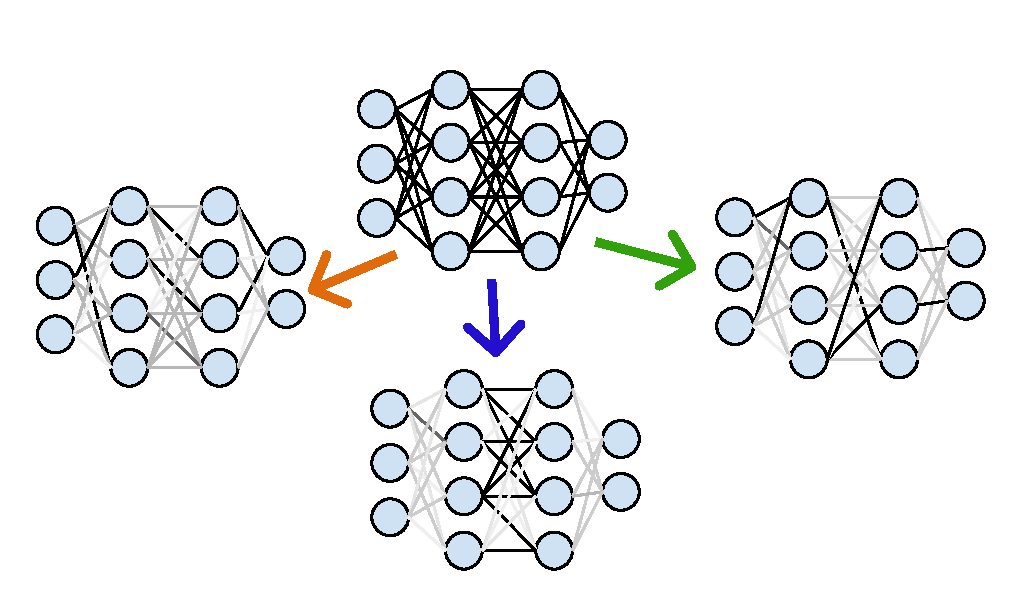
\includegraphics[width=.7\textwidth]{../figures/1b_jacobian_diagram.pdf}
    \end{subfigure}
    \begin{subfigure}{\columnwidth}
        \centering
        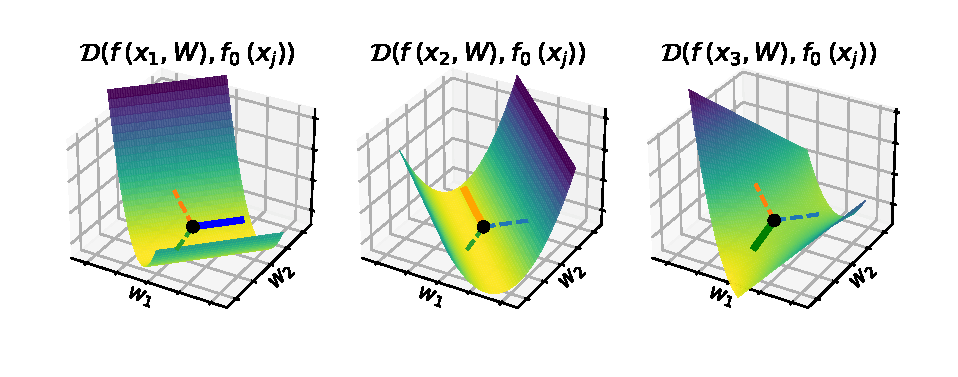
\includegraphics[width=\textwidth]{../figures/1a_jacobian_diagram.pdf}
    \end{subfigure} \caption{Decomposing a loss landscape into a set of parameter directions, or subnetworks, where a smaller subset of directions can approximately reconstruct any per-sample-pair gradient of divergence Here, $D$ is a loss, or \textit{divergence} measure, $f$ is our model, $W$ is the set of parameters in the model, $x_i$ is a sample input, and $y_r$ is our reference output}\label{fig:1_jacobian_diagram}
    
\end{figure}


\section{Methodology}\label{sec:methods}

In the next sections, we will formally set up our decomposition problem (Section \ref{sec:setup}), define the criteria that we will use for our subnetwork/parameter directions (Section \ref{sec:criteria}), describe how to efficiently decompose parameters into these directions (Section \ref{sec:decomposition}), walk through our training algorithm (Section \ref{sec:training}), and then explain how to use these decompositions to intervene on a model's behavior (Section \ref{sec:intervention}). 

From now on, we will use the word "subnetworks" to refer to the directions in parameter space we wish to learn. 

\subsection{Set up}\label{subsec:setup}


Consider a model $f$ that takes a batch of inputs $X$ and parameter values of $W$, and outputs a batch of outputs.

\begin{equation}
    f(x, W) : \mathbb{R}^{n_s \times n_f} \rightarrow \mathbb{R}^{n_s \times n_o}
\end{equation}

where $n_s$ is the number of samples in the batch, $n_f$ is the length of each input vector, and $n_o$ is the length of each output vector.

Our approach rests on the hypothesis that, for a given input, there are many components of a model's parameters that are not involved in inference. Changing parameters in the direction of these components will not affect change the model's output. Conversely, changing parameters in the direction of components that \textit{are} involved \textit{would} change the model's output. We are interested in finding parameter directions that, when perturbed, \textit{meaningfully} change a model's output.  The next subsection will explain what constitutes "meaningful".

\subsection{Divergences of Paired Outputs}\label{subsec:divergences}

To restate point (3), intervening in a relevant parameter direction should move a sample’s output either closer to or further from a reference output. This reference output should serve as a neutral and representative baseline that captures the typical behavior of the model’s output distribution. We considered three candidates for this reference:

\begin{enumerate}
    \item \textbf{A uniform output:} This reference consists of a vector with uniform values. However, it fails to account for the training distribution, leading to a bias toward learning subnetworks that influence outputs that skew toward particularly high or low values.
    \item \textbf{Mean of outputs:} This reference is computed by averaging each output across the training distribution or a batch. While it is grounded in the data, it risks averaging away meaningful correlations between outputs, producing a reference that may be out-of-distribution relative to the training data.
    \item \textbf{Another sample as the reference:} For each sample, we use the output of a randomly selected sample as the reference. This approach preserves the nuances of the output distribution but may lead to slow convergence due to high variance in reference selection.
\end{enumerate}

We thought (3) was the most principled, and least biased of the three. Although not tested rigorously, in early prototypes all three choices seemed to produce reasonable results on toy models and we did not find any issues with convergence using (3). For this work we use (3) as our reference output, but we believe other choices are possible and may have different strengths and weaknesses.

Therefore, we will decompose gradients of the loss between pairs of outputs with the aim of finding directions that move the model's output towards or away from our reference. \textbf{Because we use the term "loss" later on when we describe our training process, we will refer to this metric instead as "divergence."}

Divergence of a pair of outputs can be defined as:
\begin{align}\label{eq:divergence}
    &\nabla_W D(f(x_i, W), y_r)|_{W=W_0} \\
    &\text{ where } x_i, x_r \in X \notag
\end{align}
Here, $D$ is a divergence measure, $f$ is our model, $x_i$ is our input of interest, $y_r$ is a reference output, $W$ is a set of parameters and $W_0$ are model's original parameters. Our toy models are regression-type models, so we use MSE as divergence. For the real-world transformer and CNN models, we use KL-divergence.

We will abbreviate the expression in Eq. \ref{eq:divergence} as $\nabla_W D$.

\subsection{Sparse Principal Directions}\label{subsec:decomposition}

We want to transform our gradient into directions in parameter space, where each sample's gradient can be written as a linear combination of a small set of these components. We will do this by learning transforms $V^{in} \in R^{n_v \times n_w}$ and $V^{out} \in R^{n_w \times n_v}$ where $n_w$ is the number of parameters in the model, and $n_v$ is the number of components (subnetworks) we wish to use to represent the parameter space.

$V^{in}$ effectively transforms a gradient from the parameter space to the subnetwork space, so that: 
\begin{equation}
    \nabla_V D = V^{in} \nabla_W D
\end{equation}
We want to find $V^{in}$ and $V^{out}$ such that for any given pair of samples a small subset of subnetworks can approximately reconstruct the gradient of divergence. 
\begin{align}
    & \nabla_W D \approx V^{out} \Lambda V^{in} \nabla_W D \\\\
    & \text{where }  
    \Lambda_{i,j} = 
    \begin{cases} 
        1 & \text{if } i = j \text{ and } i \in \underset{i}{\text{argtopK}} \left[ \left| \nabla_{v_i} D \right| \right] \\ 
        0 & \text{otherwise}
    \end{cases} \\
\end{align}

$\text{topk}$ relies on a hyperparameter that controls the number of components we wish to use to reconstruct each sample. In practice, we use a $\text{batchTopK}$ \cite{bussmann2024batchtopk} and a fraction rather than an absolute number. A $\text{topK}$ of 0.1 it means that we select the top 10\% of $\nabla_V D$ magnitudes over $v$ and $x$ to reconstruct our batch of gradients.

\subsubsection{Low Rank parameter directions}
Learning a set of full rank parameter parameter directions would be extremely expensive (we would be learning $n_w n_v$ values). We also expect that modular, sparsely active circuits would be lower rank than their full-model counterparts because they are processing smaller numbers of features. Therefore, we use low-rank representations of our $V^{in}$ and $V^{out}$, and correspondingly learn low-rank circuits (Appendix \ref{sec:low_rank}). 

\subsection{Training}\label{subsec:training}
We wish to learn the decomposition-related transforms $V^{in}$ and $V^{out}$ that minimize the topK reconstruction loss of our divergence gradient described above. We use a (normalized) L2 norm loss.

\begin{equation}
    L = \frac{{|| \nabla_W D - V^{out}_{:,\mathcal{K}} V^{in}_{\mathcal{K},:} \nabla_W D ||}_2}{{|| \nabla_W D ||}_2}
\end{equation}
For each batch of samples, we randomly select a reference sample $x_r$ to be paired with each sample $x_i$ in the batch. We then compute the gradient of divergence of $x_i$ and $x_r$ at the target model's parameters $W_0$. We transform that gradient into the subnetwork space using $V^{in}$, and compute the $\text{topK}$ components. We transform those components back into the original parameter space using $V^{out}$, and compute the loss between the reconstructed gradient and the original gradient. We apply a learning update to $V^{in}$ and $V^{out}$ with the goal of minimizing this loss. We also normalize $V^{out}$ to be a unit vector after each update keep the magnitudes of $V^{in}$ and $V^{out}$ similar.


% Algorithm 1
\begin{algorithm}\label{alg:training}
\caption{Algorithm for decomposing parameter space using L3D.}
\begin{algorithmic}[1]
\FOR{each epoch}
    \FOR{each $X$}
        \FOR {each $x_i \in X$}
            \STATE Randomly select $x_r \in X$
            \STATE $\nabla_w D_i = \nabla_w D(f(x_i, W), f(x_r))|_{W=W_0}$
        \ENDFOR
        \STATE $\nabla_v D = {V^{in}} \nabla_w$
        \STATE $\tau = \text{topK}(\text{abs}(\nabla_v D))$
        \STATE $\hat{\nabla}_w D = {V^{out}} (\nabla_v D \odot (\text{abs}(\nabla_v D) > \tau))$
        \STATE $L = {|| \nabla_w D - \hat{\nabla}_w D ||}_2$
        \STATE $L.\text{backward()}$
        \STATE Update $V^{in}$ and $V^{out}$
        \STATE Normalize $V^{out}$ to be unit vectors.
    \ENDFOR
\ENDFOR
\end{algorithmic}
\end{algorithm}

\subsection{Measuring and Intervening}\label{subsec:intervention}

Our learned subnetworks will just be the rows of $V^{out}$, reorganized into the same tensor structure as $W$. After identifying subnetworks, we may want to intervene on a specific circuit.

If we wish to intervene using a single subnetwork, we can update the parameters in by moving them in a scalar factor ($\delta$) of that unit direction. To tune our model in the direction of subnetwork $v_i$ and compute predictions on $x$, we evaluate:
\begin{equation}
    f(x, W + \delta v_i)
\end{equation}


We also may want to quantify the impact of a subnetwork in on a certain sample. First, we can compute the impact of a subnetwork on a sample's ($x_i$) divergence with a reference output $y_j$. The impact of subnetwork $v_k$, $I(x_i, x_j, v_k)$ can be measured by:

\begin{equation}
    I(x_i, y_j, v_k) = \\
    \left| V^{in}_{k,:} \nabla_w D(f(x_i, W), y_j) \right|
\end{equation}

Because we are randomly sampling outputs from our training distribution as the reference output, we then average the impacts of a subnetwork $v_k$ and an input $x_i$ over many different reference samples to better quantify the impact of the subnetwork on a single sample's predictions overall. Although more computationally expensive, this gives a more robust measurement for the impact of a subnetwork on a specific sample. 

\begin{equation}
    I(x_i, v_k) = \frac{1}{n_j} \sum_{j=1}^{n_j} I(x_i, y_j, v_k)
\end{equation}

\section{Results}\label{sec:results}

To evaluate L3D's ability to decompose models, we focus on developing toy models that involve well-defined subnetworks.

We designed several toy models to test the efficacy of L3D. Our toy models all consist of several well-characterized computations being performed by the same model, with an input space designed to rely on a single or small set of tasks. 

Our toy models progressively test more complex types of circuits. Table \ref{tab:toy_models} describes our 4 toy models and the different attributes of circuitry the are designed to capture. The specific hyperparameters used to train our toy models is described in Appendix \ref{sec:toymodel_hyperparams}, as well as the hyperparameters used for each decomposition in Appendix \ref{sec:L3D_hyperparams}

\begin{table*}[htb]
    \centering
    \begin{tabularx}{\textwidth}{X X X X X}  % Adjusted for new column structure
        \toprule
         & Toy model of superposition & Circuit Superposition (TMCS) & Higher Rank Circuit Superposition & Complex Loss Landscape \\  
        \midrule

        \hline
        & 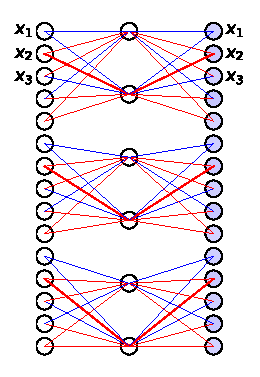
\includegraphics[width=0.12\textwidth]{../figures/2a_toy_models_setup.pdf} &
        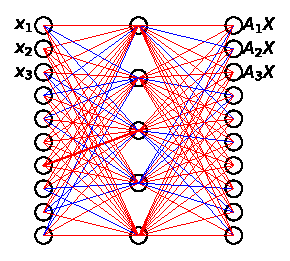
\includegraphics[width=0.2\textwidth]{../figures/2b_toy_models_setup.pdf} &
        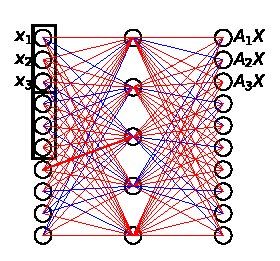
\includegraphics[width=0.2\textwidth]{../figures/2c_toy_models_setup.pdf} &
        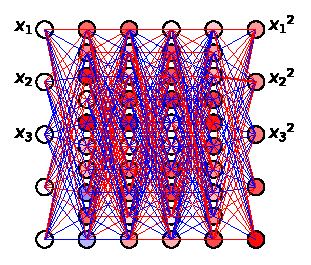
\includegraphics[width=0.2\textwidth]{../figures/2d_toy_models_setup.pdf} \\
         & $X \mapsto X$ & $X \mapsto A X$ & $X \mapsto A X$ & $X \mapsto X^2$ \\  
        Feature Superposition & $\checkmark$ & $\checkmark$ & $\checkmark$ & $\checkmark$ \\  
        Circuit Superposition & $\times$ & $\checkmark$ & $\checkmark$ & $\checkmark$ \\  
        Circuits $>$ rank-2 & $\times$ & $\times$ & $\checkmark$ & probably $\checkmark$ \\  
        Complex Loss Landscape & $\times$ & $\times$ & $\times$ & $\checkmark$ \\  
        \bottomrule
    \end{tabularx}
    \caption{Our toy models and their various properties.}
    \label{tab:toy_models}
\end{table*}

\subsection{Toy Model of Superposition}

\subsubsection{Setup}

We start off by validating our algorithm on a well-studied toy problem, the toy model of superposition (TMS). TMS is simple linear autoencoder with a low-dimensional hidden layer followed by a ReLU activation function at the output \cite{elhage2022toy}. The model is trained on a dataset of samples where few features are active at a time, and ``superimposes" these features in the hidden layer such that features embeddings in the hidden layer have minimal interference with each other \ref{fig:s2_tms_encoder_directions}. We train a toy model of superposition with 5 features and 2 hidden dimensions (with sparsity=.05) to test L3D's ability to resolve models with superimposed features.

\subsubsection{Decomposition}

We decompose the TMS model into 5 subnetworks, using rank-1 parameter tensors. The network decomposes into subnetworks as we would expect: each subnetwork represents the embedding and reconstruction of a single input element, involving only the weights connecting the relevant input and output, and the final bias. Figure \ref{fig:3_tms_subnetworks_first5} shows the decomposition. One thing to note is that parameter vectors do not have a preferred direction. L3D is equally likely to identify a parameter vector in the direction of $\theta$ as it is in the direction of $-\theta$. This is why, for example, the weights and biases in subnetwork 1 are in the opposite direction as the original network (Table \ref{tab:toy_models}).

 L3D successfully decomposes the model into subnetworks corresponding to the encoding and decoding of each feature (a $X_i:\hat{X}_i$ circuit). Moreover, the encoder directions of the learned subnetworks are nearly perfectly parallel to the original encoding of each input (Figure \TODO{ADD NEW FIGURE IN}.  This decomposition resulted in a reconstruction error of 19\%. The reconstruction error is related to the interference between features when multiple features are active in the same sample. We expect decompositions of higher dimensional networks to exhibit less reconstruction error, as the amount of nearly orthogonal parameter vectors (non-interfering) that can be compressed into parameter space scales exponentially with dimension. We see this effect in the next higher-dimensional toy model where the reconstruction loss is in fact lower. 

%--------------------- FIGURE 2: TMS Subnetworks - First 5 ---------------------
\begin{figure*}
    \centerline{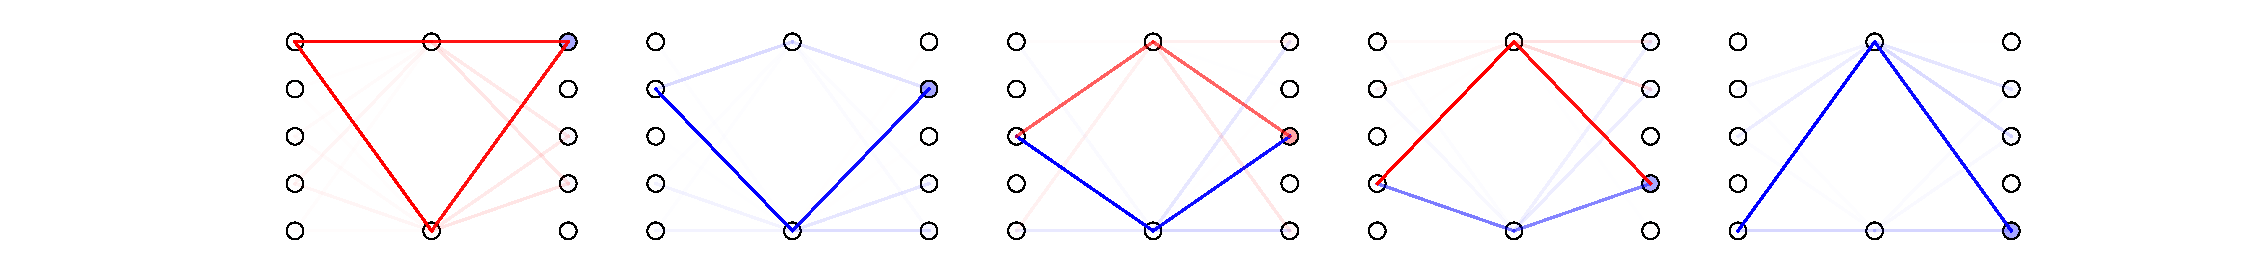
\includegraphics[width=\textwidth]{../figures/3_tms_first_5_subnetworks.pdf}}
    \centering
    \caption{L3D subnetwork decomposition of TMS}\label{fig:3_tms_subnetworks_first5}
\end{figure*}


\subsubsection{Intervention}

Parameter vectors learned by L3D can be used to intervene on model behavior. In principle, we could finetune a model using only selected subnetworks (See Appendix \ref{sec:finetuning}). While we do not go the extent of finetuning a model, we explore the effect of perturbing a model's parameter space in the direction of a subnetwork (by an increment of $\delta$), as described in Section \ref{subsec:intervention}. If subnetworks do in fact represent sparse computations, we hope that intervening on a subnetwork has a strong effect on the predictions of relevant samples, and little effect on others. As shown in Figure \ref{fig:4_tms_intervention}, moving the TMS model in the direction of a single subnetwork does in fact achieve this. Perturbing in the direction of subnetwork 1 primarily affects samples where feature 1 was active, with a small effect on the inputs that had interference to feature 1's embeddings. In fact, for TMS-in-parallel, we can successfully fully "turn off" a computation by moving far enough in the direction of the subnetwork. (Although for models with more complex loss landscapes, turning "off" a computation is not as straightforward, as we will later discuss).

%--------------------- FIGURE 4: TMS Intervention ---------------------
\begin{figure}
    \centerline{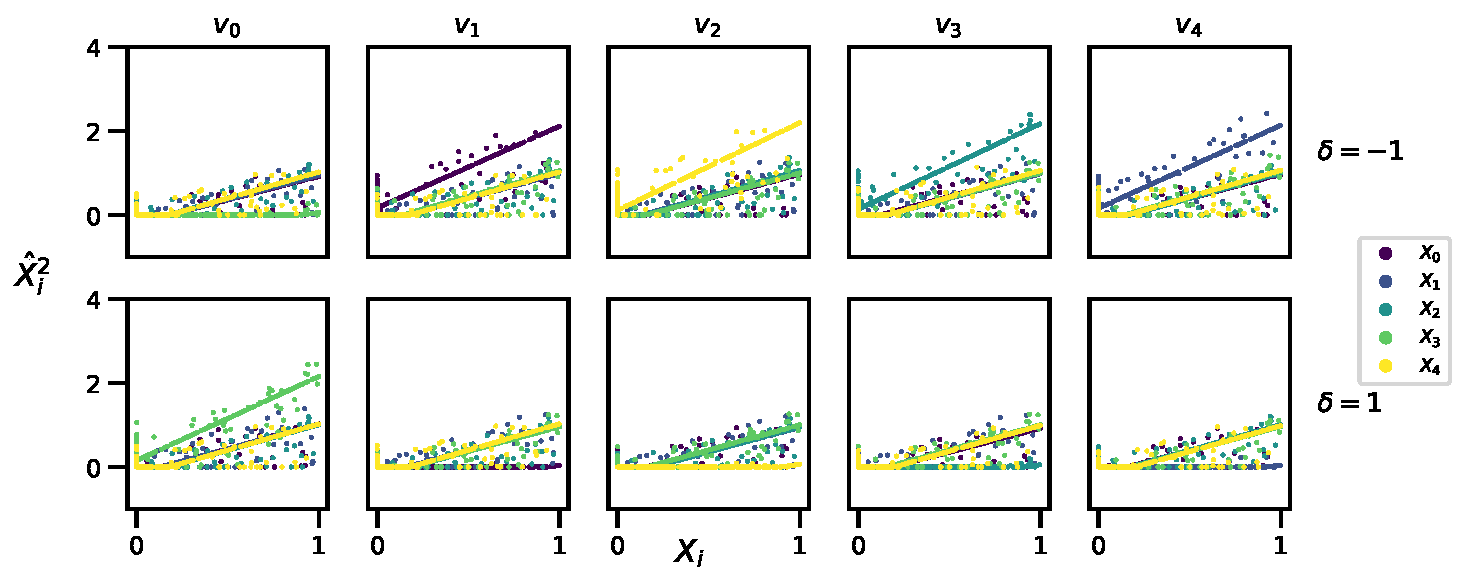
\includegraphics[width=\columnwidth]{../figures/4_tms_intervention.pdf}}
    \centering
    \caption{The effect of intervening on the TMS-in-parallel model in the direction of each subnetwork. We generate 1000 inputs from the TMS input distribution (x-axis), intervene on each subnetwork with magnitude $\delta$ (color scale) and measure the change in outputs (y-axis) for each sample.}\label{fig:4_tms_intervention}
\end{figure}

\begin{figure}
    \centerline{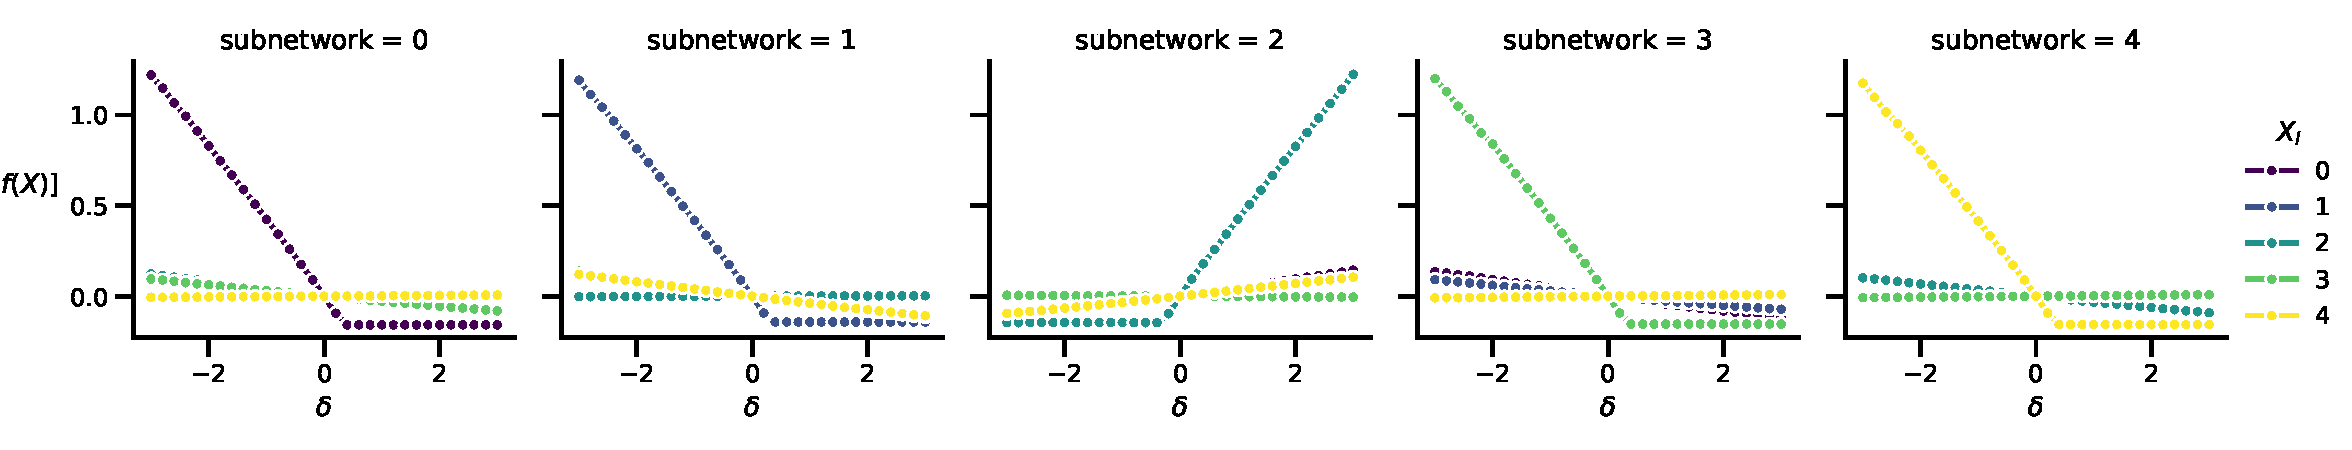
\includegraphics[width=\columnwidth]{../figures/4_tms_intervention_mean.pdf}}
    \centering
    \caption{The effect of intervening at various values of $\delta$ in the direction of each subnetwork. Each datapoint represents the average TODO FILL IN}\label{fig:4_tms_intervention}
\end{figure}

\subsection{Toy Model of Circuit Superposition}

\subsubsection{Setup}

TMS exhibits feature superposition - the input features' low dimensional embeddings are non-orthogonal. However, the sparse circuits in the original TMS we decomposed are notably \textit{not} in superposition - a given weight or parameter is only relevant for a single circuit and circuits. It seems highly unlikely that real world model circuits would decompose this way, since learning circuits composed of perfectly orthogonal parameter vectors limits the amount of circuits that can be contained in a given set of parameters. We therefore develop a toy model of \textit{circuit superposition} (TMCS) in order to analyze L3D's ability to resolve such circuits. We define circuit superposition as a phenomenon by which subnetworks share parameter elements, and even more generally have non-orthogonal parameter vectors.

Our toy model of circuit superposition (Toy model 2 in \ref{tab:toy_models})  uses the same architecture and input data distribution as TMS, but is trained to predict linear combinations of the input features as its output ($X \mapsto A X$). We set the entries of $A$  as uniform random values between 0 and 3 and generate input-output pairs to train the toy model with. We use an model with 10 inputs, 5 hidden layers, and 10 output features (although such a model does not need to have the same number of input and outputs).

If subnetworks are only relevant to a small set of inputs, then we would expect each subnetwork to be the weights and biases associated with a single input feature. If this is the case, then individual parameters would be involved in multiple subnetworks: ${W^{dec}}_{i,1}$ (the set of parameters connecting the hidden nodes to the first output node) will contain information about both $A_{1,1}, A_{2,1}, A_{3,1}...$.  Put another way, the subnetworks will interfere with each other - parameter directions associated with each subnetwork will be non-orthogonal. 

\subsubsection{Decomposition}

We decompose TMCS into 10 subnetworks of rank-1 parameter tensors (\ref{fig:5_circuit_superposition_decomposition}) with a reconstruction loss of 6.4\%. The subnetworks each strongly correspond to a single input feature, as desired.


%--------------------- FIGURE 5: Circuit Superposition ---------------------
\begin{figure*}[htbp]
    \centerline{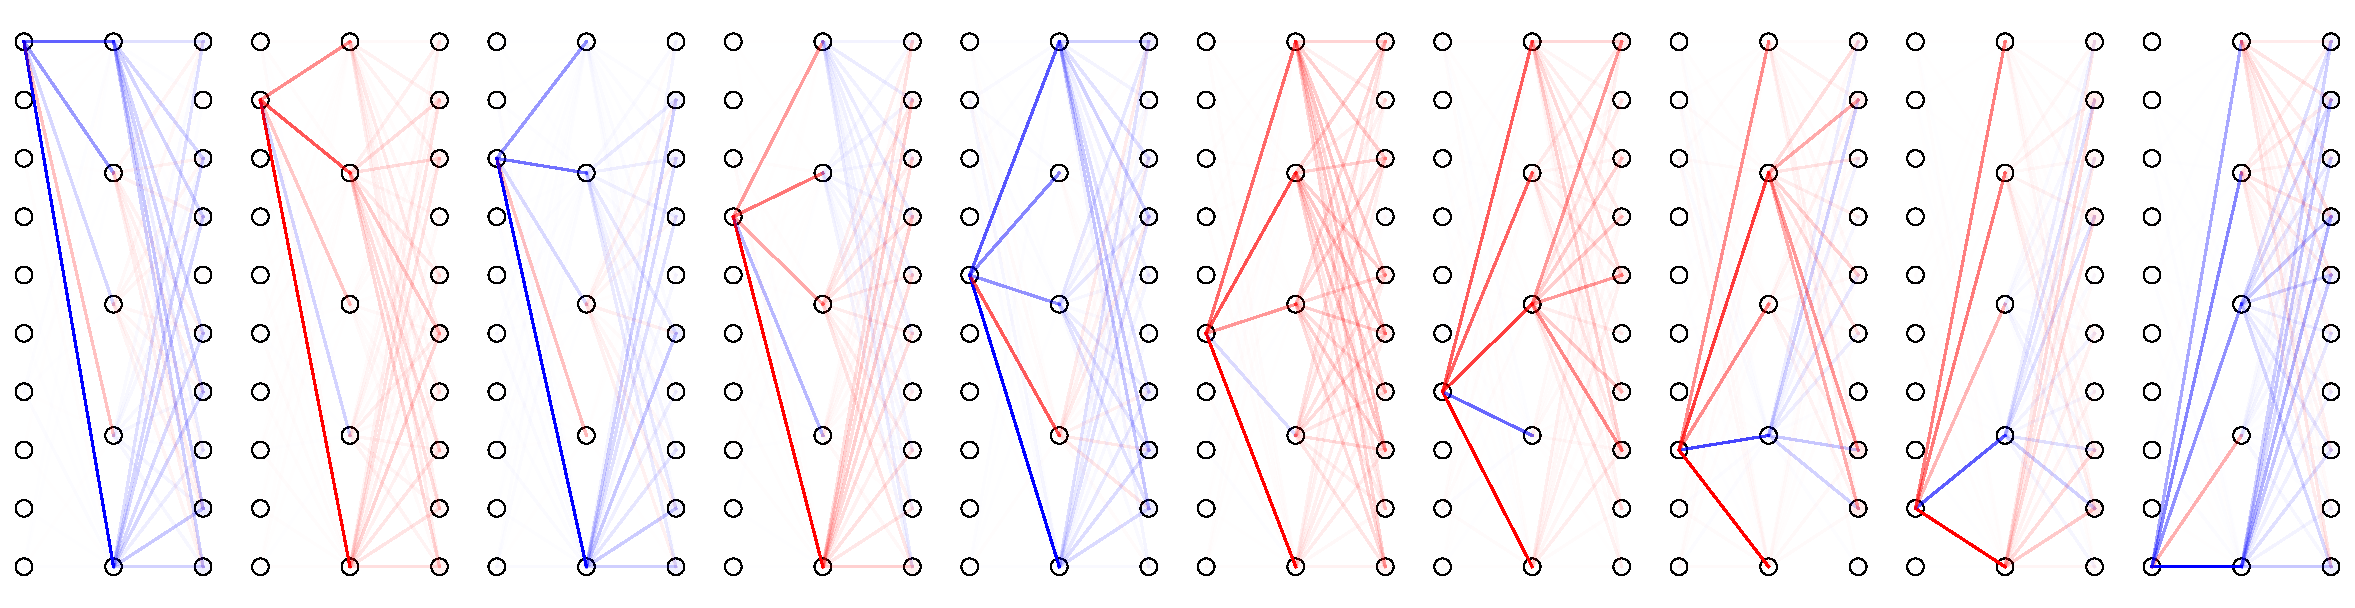
\includegraphics[width=\textwidth]{../figures/5_circuit_superposition_decomposition.pdf}}
    \centering
    \caption{The subnetworks L3D decomposes the TMCS model into.}\label{fig:5_circuit_superposition_decomposition}
\end{figure*}


Since each subnetwork theoretically corresponds to the computations involved with a single input feature, we should be able to reconstruct the original $A$ values from each subnetwork. To derive $A$ from each subnetwork, we (1) identify the which column in the subnetwork's $W^{dec}$ direction has the largest norm and then (2) trace the weights of the network through that path. That is for subnetwork $k$: 

\begin{align}
    &j^* = \underset{j}{\text{argmax}} ||{{{W^{dec}}_j}_k}||_2 \\
    &\hat{a}_{i,j^*} = {{{W^{enc}}_{i,j^*}}}_k {{W^{dec}}_{i,j^*}}_k \notag
\end{align}

Recall the parameter vectors are normalized to be unit vectors so we expect them to be a scalar multiple of the true $A$ values. As seen in Figure \ref{fig:5_circuit_superposition_decomposition}, our derived $\hat{a}$ have a very high correlation to the original $a$ values ($r^2 = 0.92$).



%--------------------- FIGURE 6: Circuit Superposition Coefficients ---------------------
\begin{figure}[htbp]
    \centerline{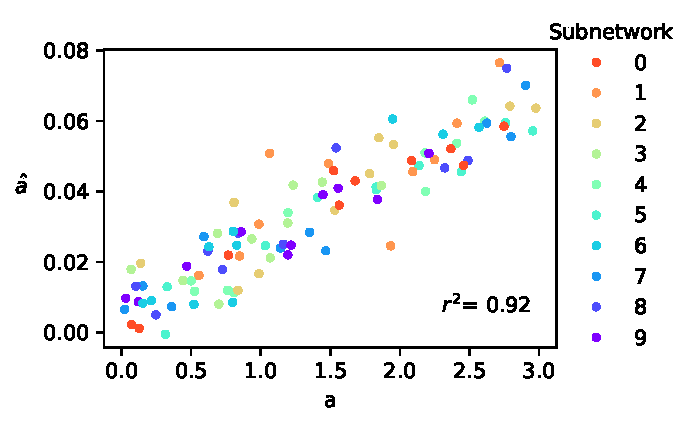
\includegraphics[width=\columnwidth]{../figures/6_circuit_superposition_coefficients.pdf}}
    \centering
    \caption{The coefficients derived from the subnetworks compared to actual coefficients used to train TMCS.}\label{fig:6_circuit_superposition_coefficients}
\end{figure}


\subsection{Higher Rank Circuits}

\subsubsection{Setup}
Because each subnetwork in TMCS traces the path of a single input neuron, the underlying subnetworks should inherently have a rank of 1. In order to test the ability of L3D to learn higher rank circuits, we developed a toy model with inherently higher rank circuits. For this model, we use the same set up as TMCS, but we correlate the sparsities of sets of input features. We use 25 input features, and we filter our data to ensure that input features 1-5, 6-10, etc, are always active ($>0$) or inactive ($<0$) together. In this setup, circuits should always be associated with groups of 5 input features and so should have a rank of 5.

\subsubsection{Decomposition}

Although we expect the model to have 5 subnetworks, we use excess parameter tensors (n=10) in order to allow more flexibility in learning. We track the fraction of inputs for which a subnetwork was used in the topK reconstruction ($P_{act}$) to identify which were ``dead circuits", and report the last epoch. Futhermore, although we expect the underlying subcircuits to be rank 5, we experiment with using different rank representations to see how well lower-rank parameter directions can represent the model. Interestingly, rank-1 representations of the parameter tensors are able to represent the model nearly as well as rank-5 representations (Figure \ref{fig:s5_high_rank_circuits_loss_vs_rank}). In Figure \ref{fig:7_high_rank_decomposition}, we show the decomposition of a rank-3 decomposition. L3D successfully learns a subnetwork corresponding to each of the 5 sets of input features, as well as a number of dead circuits. The higher and lower rank decompositions also learn similar subnetworks (Figure \ref{fig:s6_high_rank_decompositions}). When we trained L3D without these additional subnetworks, the reconstruction loss gets caught in local minima. Similar to training sparse autoencoders \cite{cunningham2023sparse}, having extra degrees of freedom allows for better learning, even if at the end of training the extra subnetworks are never active.


%--------------------- FIGURE : Higher Rank Circuit Superposition ---------------------
\begin{figure*}[htbp]
    \centerline{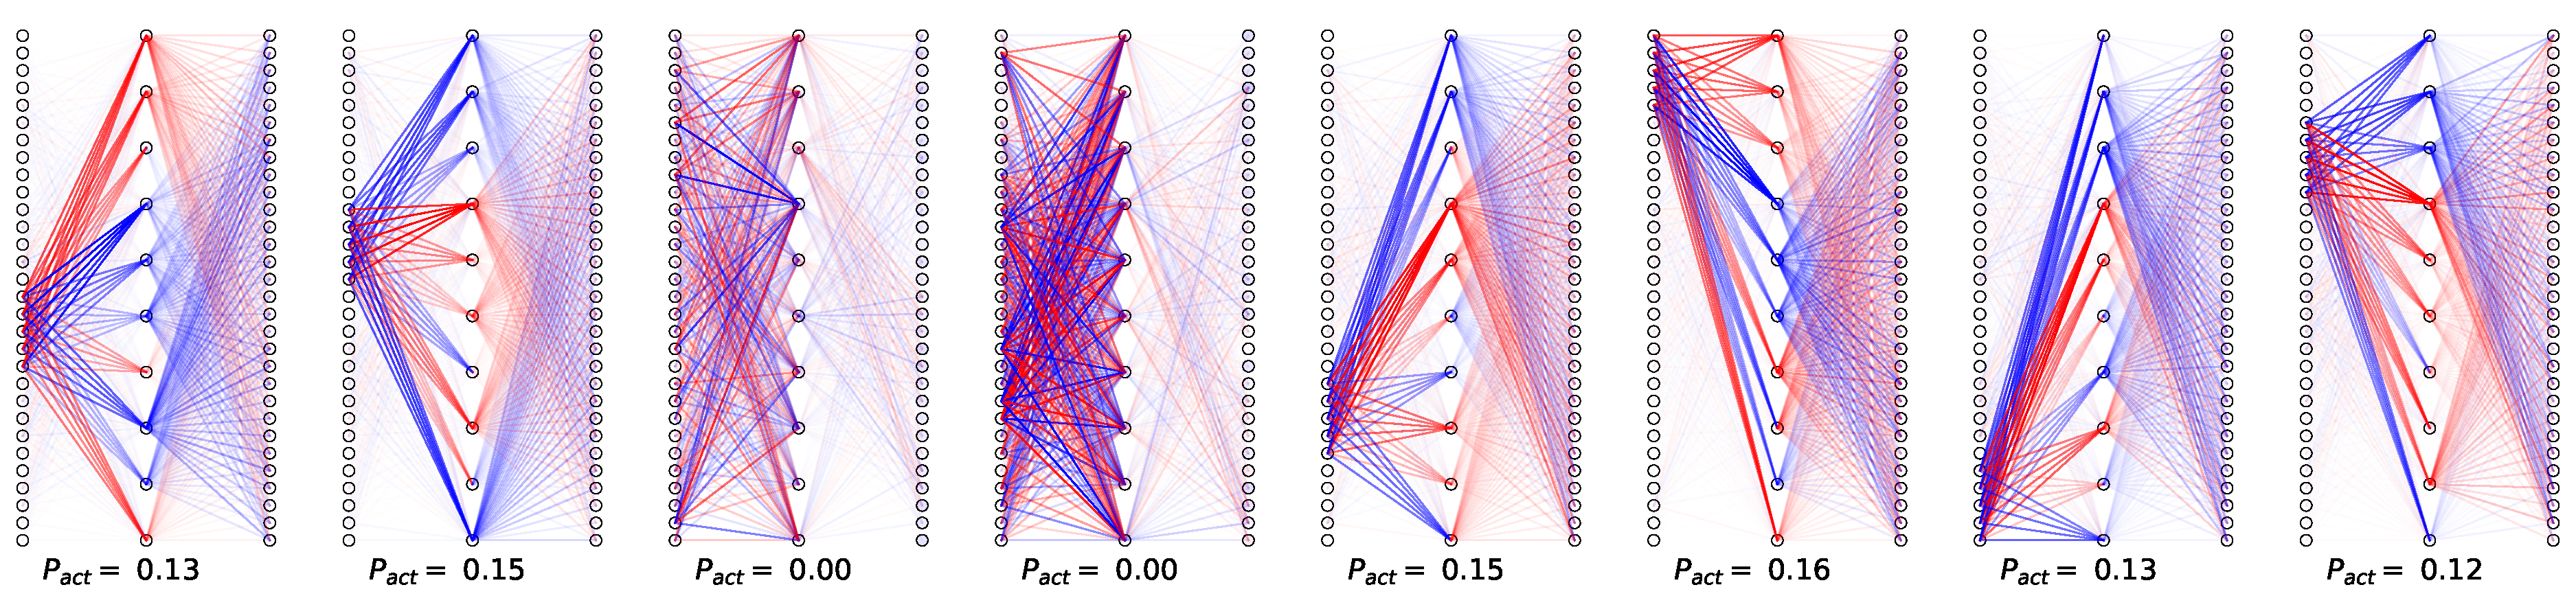
\includegraphics[width=\textwidth]{../figures/7_high_rank_decomposition.pdf}}
    \centering
    \caption{Parameter representations learned by L3D for the high rank circuit decomposition task.}\label{fig:7_high_rank_decomposition}
\end{figure*}


\subsection{Toy model with Complex Loss Landscape}


\subsubsection{Setup}

In the previous models, assuming the the final layer ReLUs have fired, the gradient of divergence with respect to  to an element of $W^{dec}$ looks like:
\begin{equation}
  \nabla_{W^{dec}_{i,j}} ( X W^{enc}W^{dec} + b - X)^2 = (2 (X W^{enc} W^{dec} + b- X)^T X W^{enc})_{i,j}
\end{equation}
The gradient is linear with respect to $W^{dec}$. With this gradient, we expect local approximations to be excellent approximations of global loss landscapes (up until the Relu-induced discontinuities.) We should be able to move relatively far in parameter space (large \delta in Figure. \ref{fig:4_tms_intervention}) and see well behaved effects on predictions. However, we wanted to test the limitations of a L3D on a model with a more complex loss landscape, especially when it comes to intervening with a subnetwork.

We therefore trained a multi-layer model to predict multiple non-linear functions of input features at once. We train a GeLU network for $X_i \mapsto X_i^2$. We use a network with 4 hidden layers of 5 neurons each, and 5 input and output neurons. Once again, the input features are sparse, incentivizing the toy model to learn circuits in superposition whose interferences will cause minimal errors on the sparse input distribution. 

We expect the model to have 5 subnetworks, one for each input feature. Although it is less clear what rank the tensors of the underlying circuits should be, there are not inherent reasons to believe subnetworks should be low rank, the way there was in the TMS model. 

\subsubsection{Decomposition}

To allow for slightly higher rank subnetworks but still compress the dimensions of the model, we decompose our model into 5 rank-2 parameter tensors in our decomposition. Additionally, instead of varying rank, we experiment with using different numbers of subnetworks to represent our model. In the 5-subnetwork decomposition (Figure \ref{fig:8_squared_subnetworks}), we see that subnetworks tracing the path of $X_i \mapsto X_i^2$ for each index $i$. However, this decomposition has a relatively high reconstruction error of 0.32. Much of this is probably because we kept our $\text{topK}$ hyperparameter constant (at $k=0.1$) throughout all our our models for consistency.  With only 5 subnetworks, this means that each sample's reconstruction will use <1 subnetwork on average,  limiting the reconstruction error the network can achieve. 

We also experiment with holding rank constant (we drop to rank-1 for this) and decompose the model into different numbers of subnetworks (3, 5, 10, and 15 subnetworks). In our 3-subnetwork decomposition, L3D still learned subnetworks corresponding to single input features, but can of course only represent 3 out of the 5 inputs. As we add more subnetworks, we are able to successfully learn more expressive decompositions of the model that reduce reconstruction error (Figure \ref{fig:s11_squared_features_vs_loss}). Each decomposition continues to learn input-output pair specific subnetworks, with the larger decompositions resulting in a few more dead subnetworks as well (Figure \ref{fig:s10_squared_decompositions_features}).

%--------------------- FIGURE 8: Squared Model Subnetworks ---------------------
\begin{figure*}[htbp]
    \centerline{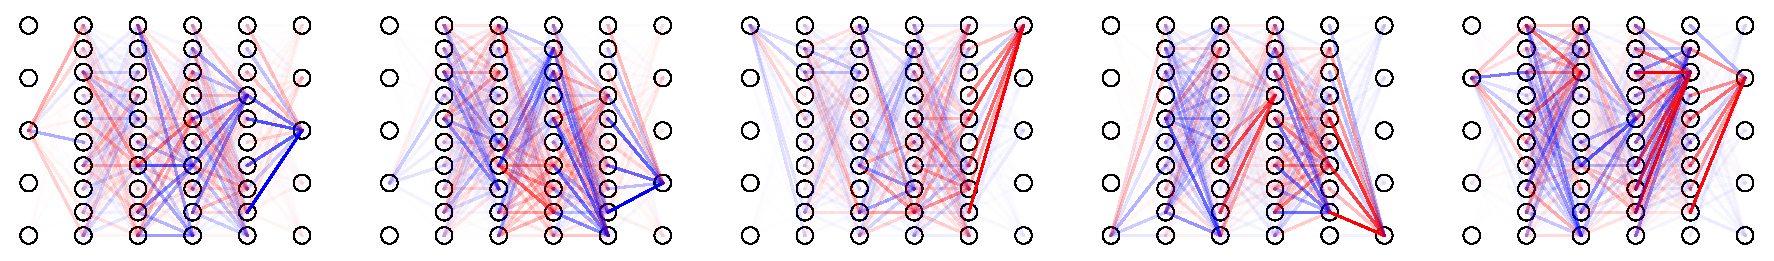
\includegraphics[width=\textwidth]{../figures/8_squared_subnetworks.pdf}}
    \centering
    \caption{Subnetworks learned by L3D for the $X \mapsto X^2$ model/}\label{fig:8_squared_subnetworks}
\end{figure*}


\subsubsection{Intervention}

Intervening on these circuits helps us understand how much local loss landscape is representative of global loss landscape, particularly when it comes to inactive subnetworks remaining inactive as we move through parameter space. If local loss landscape is truly representative of global loss landscape in this way, then intervening on on a single subnetwork should result in only a consistent small number of samples being affected, even if we move very far in that direction. Figure \ref{fig:9_squared_intervention} shows our results for these interventions. Even in this more complex toy model, local loss landscape is a relatively good approximation of the global loss landscape. We can perturb the parameters in a direction of interest and have a large impact on the predictions of that sample and a minor impact on others. If we perturb far enough (Figure \ref{fig:s7_squared_intervention_more_deltas}), we do begin to see effects on the predictions of other samples, but ratio of change in predictions to the relevant samples to those of the irrelevant samples is very high.



%----------------- FIGURE 9: Squared Subnetworks Intervention ------------------
\begin{figure*}[htbp]
    \centerline{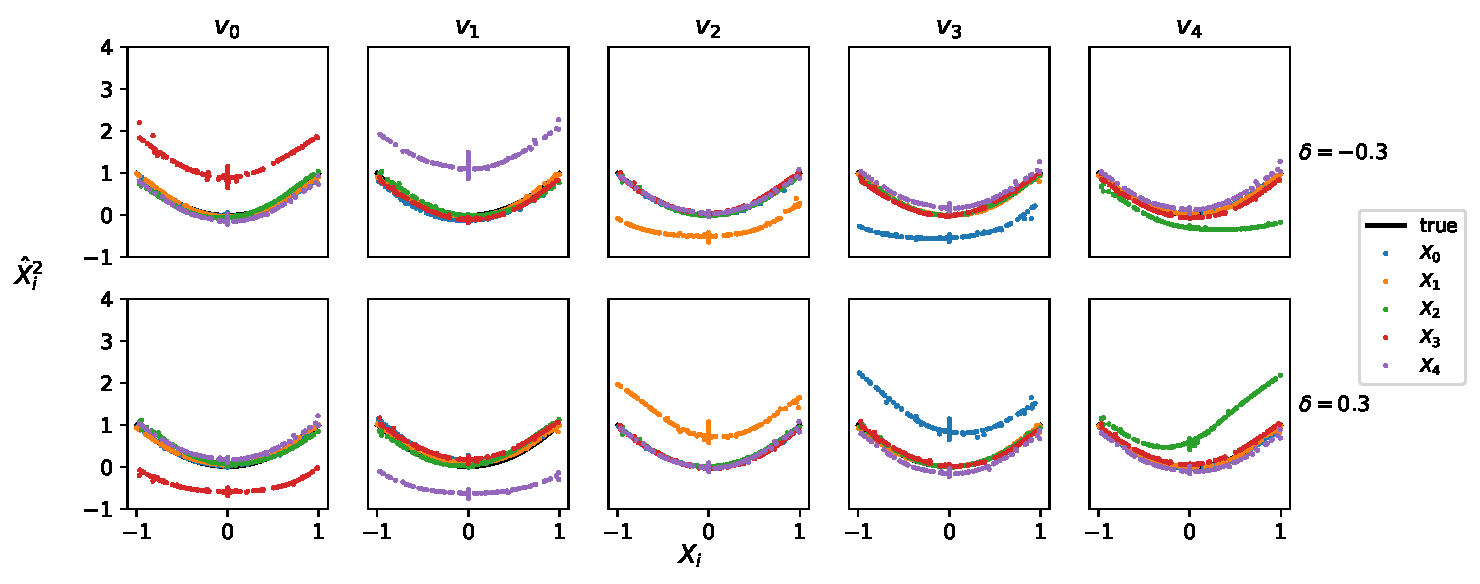
\includegraphics[width=\textwidth]{../figures/9_squared_intervention.pdf}}
    \centering
    \caption{The effect of intervening on each subnetwork in the $X \mapsto X^2$ model. We generate 1000 inputs from the TMS input distribution, intervene on each subnetwork with magnitude $\delta$ and measure the change in outputs for each sample.}\label{fig:9_squared_intervention}
\end{figure*}

Figure \ref{fig:9_squared_intervention} shows changes in predictions as we move in a single direction in parameter space. We also wanted to understand how subcircuits might interact with each other as we move through parameter space. In \ref{fig:s9_squared_intervention_multi_features} we perturb multiple subnetworks at once, and measure the new predictions. For the most part, the subnetworks have little inference with each other: the relevant output values for each subnetwork move relatively independently of each other. For some parameter directions, we do see some unexpected interactions, such as when we move in the direction of subnetwork 1 and 2, we see a small effect on the predictions of a few samples not associated with either subnetwork. With larger models, especially those with more modular circuits that are working together, we expect this kind of interaction to become more common. We discuss more in the discussion section. 

A careful reader may have noticed is that it would be very easy to identify parameter directions in the first or last layer of the $X \mapsto X^2$ model involved in a sparsely active subnetworks. For example, 5 subnetworks that each only involved one of the biases in the final layer could give similar intervention results as in Figure \ref{fig:9_squared_intervention} In order to make sure L3D is not just learning this trivial solution, we want to test if the hidden parameter directions it learns are also truly involved in the subnetwork. Therefore, we perform the same intervention experiments but only intervening with the subnetwork components related to the model's hidden layers' weights and biases (\ref{fig:s8_squared_intervention_middle_weights}). The results are very similar to  Figure \ref{fig:9_squared_intervention}, where inventions on a subnetwork only successfully affect the expected subset of outputs. 


\subsection{Real world models}

Finally, to show the promise of this method to pull out relevant features from real world models, we use L3D to decompose blocks of a language model and computer vision model.  These results are primarily qualitative, and were run with minimal compute and little hyperparameter tuning. Our choices for model block, number of subnetworks, and subnetwork rank were relatively arbitrary.  

These models do not have well-characterized subnetworks the same way our toy models do. To briefly analyze the function of the subnetworks we identify, we look at the top samples that each subnetwork is relevant to.  We compute this metric by:


\subsubsection{Language Model}

We decompose attention block 7 of the tiny-stories-8M model.  We chose an attention block because this has been a challenging component of a transformer for SDL to extract features from \cite{}, and we chose a middle layer of the model so that we identify subnetworks that are neither so high level that they line up  with next-token prediction, and not so low-level that they line up with token id. We decompose 

TODO(image with 10 features that we like)
TODO(image with more features for supplementary)


\subsubsection{Computer Vision Model}

We decompose convolutional block 4 of the mobilenet-v3-small model.  Once again we choose a middle layer such that the subnetworks we identify are neither involved in low-level computations that would likely require additional pixel attribution methods to interpret, or so high level they perfectly line up with classification. 

TODO(image with 10 features that we like)
TODO(image with more features for supplementary)

\section{Discussion}

L3D is one of the earliest parameter-based decomposition methods. For this reason, we have focused our work on demonstrating the fundamentals of L3D on toy models, and showcasing its promise with more complex models. Here we discuss what we believe are simple improvements to L3D that could enhance its performance and real-world use cases to which to extend L3D. Finally, we discuss unresolved challenges and limitations of L3D. 

\subsection{Simple Improvements}
In this work, we did not focus on optimizing L3D, and we chose nearly identical hyperparameters for all of our decompositions. 

\textbf{Hyperparameter Choice}: For all of our toy model decompositions, we always chose our $\text{topK}$ hyperparameter as $k=0.1$, even when it was clear that certain toy models should have larger numbers of subnetworks activated per sample than others (For example, the $X \rightarrow X^2$ model with 5 inputs and 5 outputs, decomposed into 5 networks, should probably have $k \geq 0.2$). Too low of $k$ choice is likely responsible for the high reconstruction loss of some of our models. Similarly, we always chose the ranks of the subnetworks somewhat arbitrarily. Some preliminary research aims to understand the relationship between rank, compressibility, and interference of subnetworks \cite{hanni2024mathematical,bushnaq2024circuits}, and a better understanding of this relationship could help us choose better hyperparameters for L3D. 

\textbf{Flexible Rank Choices}: Relatedly, the way L3D makes circuit decomposition computationally feasible is to represent each tensor in the subnetwork as a low-rank tensor. For simplicity, we use the same rank for all tensors. Theoretically, there could be more flexibility across tensors, and we could use different ranks for different blocks of the subnetwork if we believed certain parts of the model were composed of fundamentally higher rank circuits. 

\textbf{Scaling up}


\subsection{Extensions}

There are a also some higher effort extensions to L3D that may give it more real-world relevance. 

\textbf{Finetuning}: Our intervention experiments showed promise subnetworks of L3D could be perturbed in ways that only affect the predictions of relevant samples. As we described in Section \ref{sec:finetuning}, this could be taken one step further by finetuning a model on a specific set of parameter directions. Using L3D networks, we could finetune a model on a specific set of parameter directions by freezing the current set of weights and learning an adapter consisting of linear combinations of the subnetworks of choice. This could also benchmark the intervention capabilities of L3D versus other mechanistic intervention strategies such as SDL-derived steering vectors. For example, we might use L3D to identify various subnetworks involved in sycophancy, refusal, and other undesired behaviors. After collecting curated data with the goal of finetuning away such behaviors, we could finetune L3D only in the direction of the behavior-related subnetworks and test how well the model achieves our desired output compared to other intervention strategies. 

\textbf{Identifying Specific Circuits with Contrastive Pairs}:
We developed this method as an unsupervised decomposition method, with goals comparable to those of SDL. However, the methods of L3D could be easily modified to use supervised signals to identify specific circuits of interest. Rather than using gradients of divergence of random pairs, we could decompose gradients of divergence between curated pairs of samples that isolate a behavior of interest. In this context, we could probably not require the topK constraint, but instead look decompose the network into a very small number of low-rank subnetworks involved in our behavior of interest. 

\subsection{Challenges}
Although many of the improvements and extensions of L3D are highly addressable, we think there are some fundamental challenges with parameter-based decomposition methods that may not be easily resolved.


\textbf{Local Attribution}: L3D's algorithm hinges on the somewhat surprising phenomenon that local gradient approximations work reasonably well as attribution methods. They clearly work well in the toy models we used for L3D and for the circuits we found in our real world models. However, do they work for all circuits? In our work, we use a randomly selected sample to be our "reference" output with which to compute divergence gradient. By using a randomly selected sample, rather than a single "reference output" such as the mean of the output distribution, we hope that the random noise in the reference sample will average out the effects of any non-convexity in the loss landscape.  However, perhaps even in this setup there are parameter directions that are highly non-convex on which it will be difficult to perform local attribution. Quantifying different types of "dark matter" of parameter decomposition by analyzing reconstruction loss (similar to recent work, such as \cite{engels2024decomposing}, done on SDL) could better help us characterize these limitations.

\textbf{Relationship to overparameterized models}: Going one step further, we suspect that the reason local attribution methods work so well is because large models are probably overparameterized \cite{kawaguchi2016deep,choromanska2015loss,dauphin2014identifying,soudry2017exponentially}. Larger models may have wider loss basins, or more degeneracies near their global minima \cite{keskar2016large,sagun2017empirical}, making local attribution methods less likely to break down as we move through parameter space. If in the future, an learning algorithm is developed that has fundamentally different limitations that stochastic gradient descent and its relatives, we might lose this property. Moreover, circuit activations might no longer be sparse. A new learning process might be able to compress subnetworks in such a way that subnetworks have very high levels of interference with each other - removing the degeneracy assumption that underlies L3D. 

\textbf{Interpretation of a circuit}: Finally, we should address the definition of ``circuits". It is still not well agreed upon what a ``feature" is in relation to large networks, and the definition of what should constitute a circuit or subnetwork is even less clear. Is our definition of a circuit - sparsely active subnetworks that can move outputs within the original output distribution - too restrictive? If there is a circuit that is relevant to every output, a sort of ``scaffolding" for more specific circuits - should it be included in the decomposition? If, after identifying the structure of subnetworks, we cannot interpret it beyond a description of its end results, are circuits any more informative than they features they are computing? If parameter decomposition is a viable strategy for understanding and intervening with large networks, these questions will be important for the mechanistic intepretability community to address.

\clearpage

\section{Impact Statement}

This paper presents work whose goal is to advance the field of neural network intepretability. There are many potential societal consequences of our work, none which we feel must be specifically highlighted here.

% In the unusual situation where you want a paper to appear in the
% references without citing it in the main text, use \nocite

\clearpage
\bibliography{writeup.bib}
\bibliographystyle{icml2025}


%%%%%%%%%%%%%%%%%%%%%%%%%%%%%%%%%%%%%%%%%%%%%%%%%%%%%%%%%%%%%%%%%%%%%%%%%%%%%%%
%%%%%%%%%%%%%%%%%%%%%%%%%%%%%%%%%%%%%%%%%%%%%%%%%%%%%%%%%%%%%%%%%%%%%%%%%%%%%%%
% APPENDIX
%%%%%%%%%%%%%%%%%%%%%%%%%%%%%%%%%%%%%%%%%%%%%%%%%%%%%%%%%%%%%%%%%%%%%%%%%%%%%%%
%%%%%%%%%%%%%%%%%%%%%%%%%%%%%%%%%%%%%%%%%%%%%%%%%%%%%%%%%%%%%%%%%%%%%%%%%%%%%%%
\newpage
\appendix
\renewcommand{\thefigure}{S\arabic{figure}}  % Set figure numbers to S1, S2, etc.
\renewcommand{\theHfigure}{S\arabic{figure}} % Fix hyperlinks in hyperref
\setcounter{figure}{0}  % Reset numbering
\onecolumn


\section{Definitions}

\subsubsection{Dimensions}
$n_s$: The number of samples in a batch of inputs 

$n_f$: The dimensions of a single input vector to a model

$n_o$: The dimensions of a single output vector from a model

$n_w$: The number of parameters values in a model.

$n_v$: The number of subnetworks or parameter directions chosen to decompose a model. 


\subsubsection{Model Syntax}
$X \in \mathbb{R}^{n_s \times n_f}, x \in \mathbb{R}^{n_f}$: Batch and individual input vectors to a model.

$W \in \mathbb{R}^{n_w}, w \in \mathbb{R}$: The set of and individual parameter values of a model

$\mathcal{w}$: The set of parameters corresponding to a specific tensor or block in a model.

$f: \mathbb{R}^{n_s \times n_f} \mapsto \mathbb{R}^{n_s \times n_o}$: A model mapping a set of input vectors to a set of output vectors.

$f(X, W)$: The output of model $f$ with parameter values $W$ on input $X$.

$f(X, W_0)$ or $f(X)$: The output of model $f$ with fixed parameter values $W_0 $. $W_0$ is the set of learned parameter values from model training.

$D$: Divergence metric between two vectors. Typical divergence metrics are mean-squared error for regression-type outputs, and KL-divergence for probability-type outputs. 

\subsubsection{Decomposition Syntax}
$V (or V^{out}) \in \mathbb{R}^{n_v \times n_w}, v (or V^{out})  \in \mathbb{R}^{n_w}$: The set of or individual parameter directions that are used to decompose a model. $V_out$ can be used to transform parameter directions in the subnetwork vector space back into the original parameter space of the model. The terms parameter direction, subnetwork, and circuit all have the same meaning. 

$\mathcal{V}_{out}, \mathcal{v}_{out}$: Components of $V^{out}$ or $V^{out}$ related to a specific tensor or block in the original model. 

$V^{in} \in \mathbb{R}^{n_w}, V^{in} \in \mathbb{R}$: Transforms the original parameter space of the model into the subnetwork vector space. 

$\mathcal{V}_{in}, \mathcal{v}_{in}$: Components of $V^{in}$ or $V^{in}$ related to a specific tensor or block in the original model. 

$r$: The rank of each component of the decomposition vectors corresponding to tensors in the original model. 

\subsubsection{Training}

$\mathcal{K}$: The subset of indexes >= $\tau$ where $\tau$ is the threshold computed by using the top $k$ absolute values in a tensor. 

$L$: The L2 reconstruction loss used to optimize $V^{in}$ and $V^{out}$.

\subsubsection{Measuring and Intervention}
$I(x_i, x_j, v_k), I(x_i, v_k)$: The impact of subnetwork $v_k$ on the divergence between samples $x_i$ and $x_j$, or averaged across many $x_j$ reference samples.

$\delta$: A scalar value to move $W$ in a specific direction. 


\section{Additional Methods}

\subsection{Low-Rank Tensor Representation}\label{sec:low_rank}

We use low-rank representations of our $V^{in}$ and $V^{out}$, and correspondingly learn low-rank circuits.

While $W$ is a vector of all of the parameters in a model, typically model parameters are organized into tensors $W=\{w_i\}_i$. 

If our parameters are organized into tensors $W=\{w_i\}_i$, each subnetwork or parameter component can be organized as $V^{in}_i  = {\{{v^{in}}_i\}}_i, V^{out}_i = {\{{v^{out}}_i\}}_i$ where we have parts of our subnetworks corresponding to each tensor in the original model parameters. We wish each of these tensors to be low rank, and we express them using the canonical polyadic decomposition \cite{} (a way to write 3+ dimentinoal tensors in terms of low-rank components).

\begin{equation}
{v^{in}}_{i,j} = \sum_{r=1}^{R} a_{i,j,r} \times b_{i,j,r} \times c_{i,j,r} ...
\end{equation}

Where $R$ is the rank we wish to use to represent the parameter component, and the number of factors (a, b, c,...) in the factorization is equal to the number of dimensions in the tensor $w_i$.

\subsection{Finetuning}\label{sec:finetuning}

To finetune a model on a specific set of parameter directions, we would freeze the current set of weights and learn an adaptor consisting of linear combinations of the subnetworks of choice. During fine tuning, we would only need to learn the coefficients of these linear combinations greatly reducing cost.

\begin{align}
    f(X, W_0 + W_{ft} V^{out}_\mathcal{I})\\
    \text{where} W_0 \in \mathcal{R}
    
\end{align}



\subsection{Toy Model Training}\label{sec:toymodel_hyperparams}

For all of our toy models (except the $X \mapsto X^2$ model), we generate uniformly random inputs between 0 and 1. For $X \mapsto X^2$, we generate uniformly random inputs between -1 and 1. For all toy model data, we use a sparsity value of 1-sparsity=.05. We generate 10000 datapoints and train for 1000 epochs with batch sizes of 32. We use an AdamW optimizer with a learning rate of 0.001. 

\subsection{L3D Model Training}\label{sec:L3D_hyperparams}

To train L3D, we use the same training distributions as in each toy models. Although optimal hyperparameter values probably depend on the model size, and the rank and number of parameter tensors, we use the same hyperparameters for all of our models. We generate only 1000 datapoints, with a batch size of 32, and train for 1000 epochs. We use an AdamW optimizer with a learning rate of 0.01, and a learning decay rate of .8 every 100 steps. We always use a $\text{topK}$ hyperparameter of $k=0.1$.  We include all of the model's parameter tensors, including biases, in the decomposition. 

\section{Supplemental Figures}


% ---------------------Figure S1 TMS subnetwork decomposition-------------------------
\begin{figure}[ht]
    \centerline{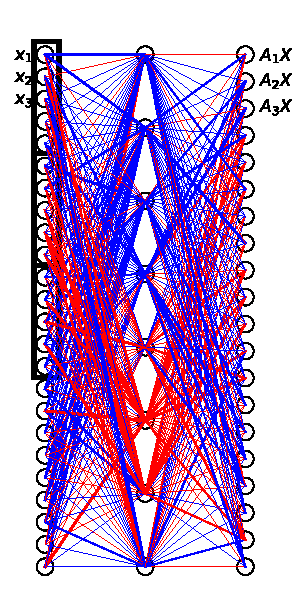
\includegraphics{../figures/s1_high_rank_circuit_setup.pdf}}
    \centering
    \caption{The full architecture of high rank circuit toy model (model C).}\label{fig:s1_high_rank_circuit_setup}
\end{figure}



% ---------------------Figure S2 TMS subnetwork decomposition-------------------------
\begin{figure}[ht]
    \centerline{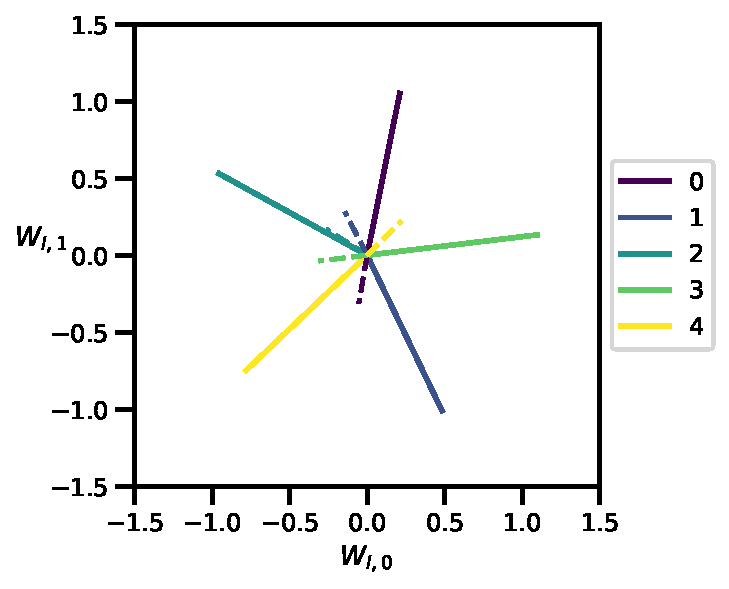
\includegraphics{../figures/s2_tms_encoder_directions.pdf}}
    \centering
    \caption{Encoder directions in the hidden layer dimension of the TMS toy model.}\label{fig:s2_tms_encoder_directions}
\end{figure}


% ---------------------Figure S2 TMS subnetwork decomposition-------------------------
\begin{figure}[ht]
    \centerline{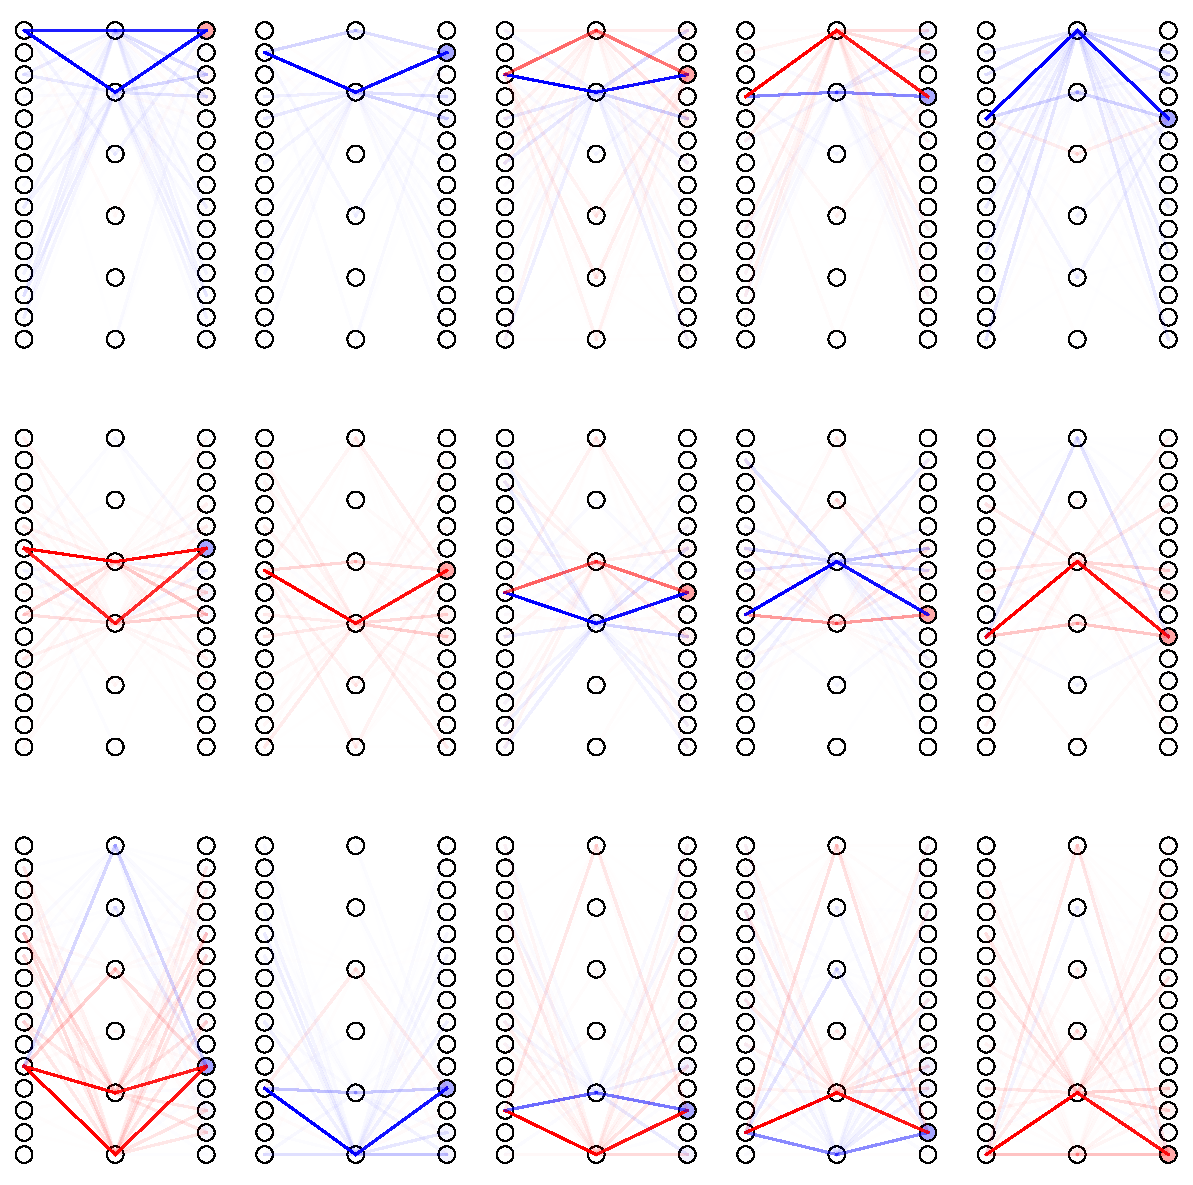
\includegraphics[width=\textwidth]{../figures/s3_tms_full_subnetworks.pdf}}
    \centering
    \caption{All subnetworks for the TMS decomposition}\label{fig:s3_tms_full_subnetworks}
\end{figure}


% ---------------------Figure S3: Intervention on TMS-in-parallel-------------------------
\begin{figure}[ht]
    \centering
    \caption{Effects of intervening on the first 5 subnetworks of the TMS-in-parallel model.}
    \label{fig:s3_tms_interventions}

    \begin{minipage}{\textwidth} % Ensure figures align
        \centering
        \begin{tabular}{cc}  % 3 columns
            \begin{subfigure}{0.3\textwidth}
                \centering
                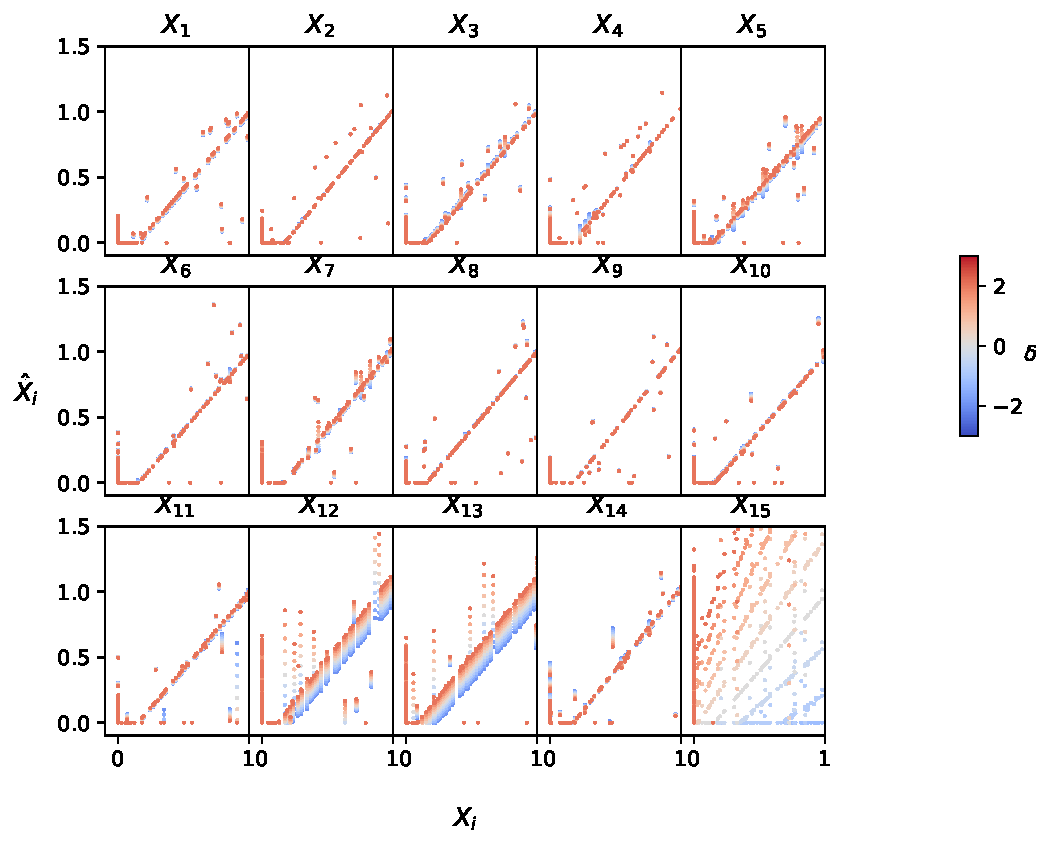
\includegraphics[width=\linewidth]{../figures/s4_tms_intervention_network1.pdf}
                \caption{Subnetwork 1}
            \end{subfigure} &
            \begin{subfigure}{0.3\textwidth}
                \centering
                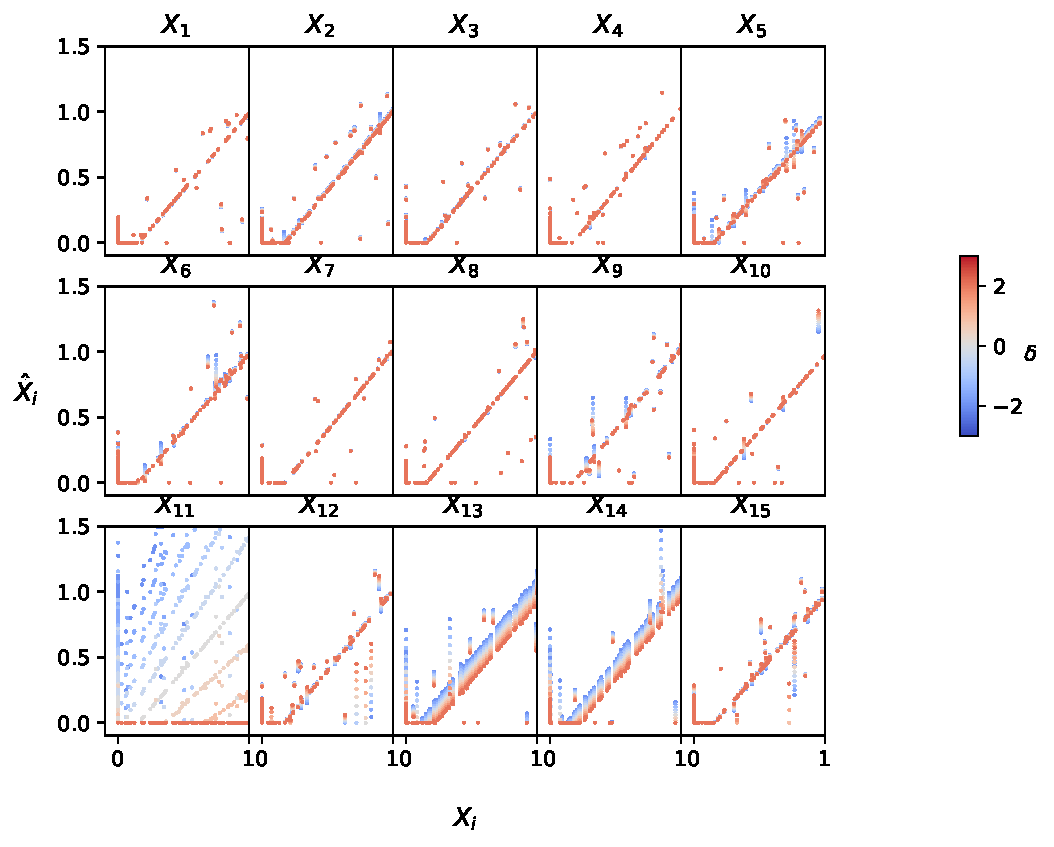
\includegraphics[width=\linewidth]{../figures/s4_tms_intervention_network2.pdf}
                \caption{Subnetwork 2}
            \end{subfigure} \\ % Move to the next row
            \begin{subfigure}{0.3\textwidth}
                \centering
                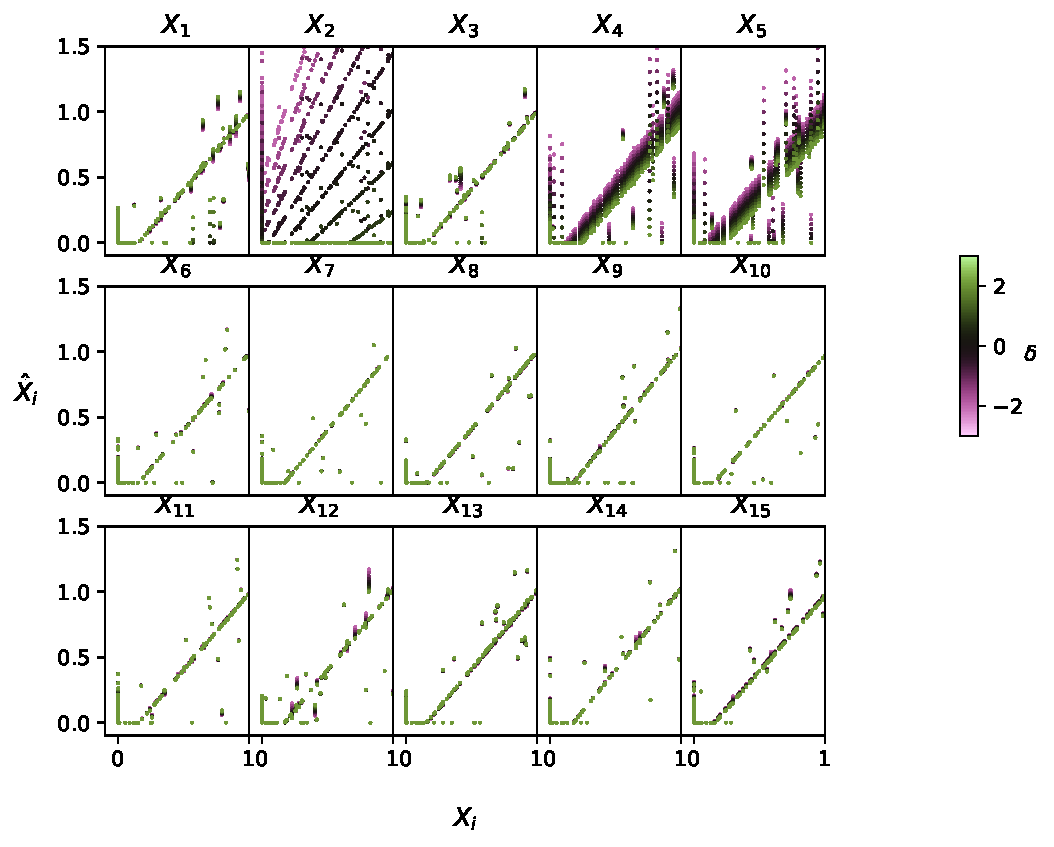
\includegraphics[width=\linewidth]{../figures/s4_tms_intervention_network3.pdf}
                \caption{Subnetwork 3}
            \end{subfigure} & % Move to the next row
            
            \begin{subfigure}{0.3\textwidth}
                \centering
                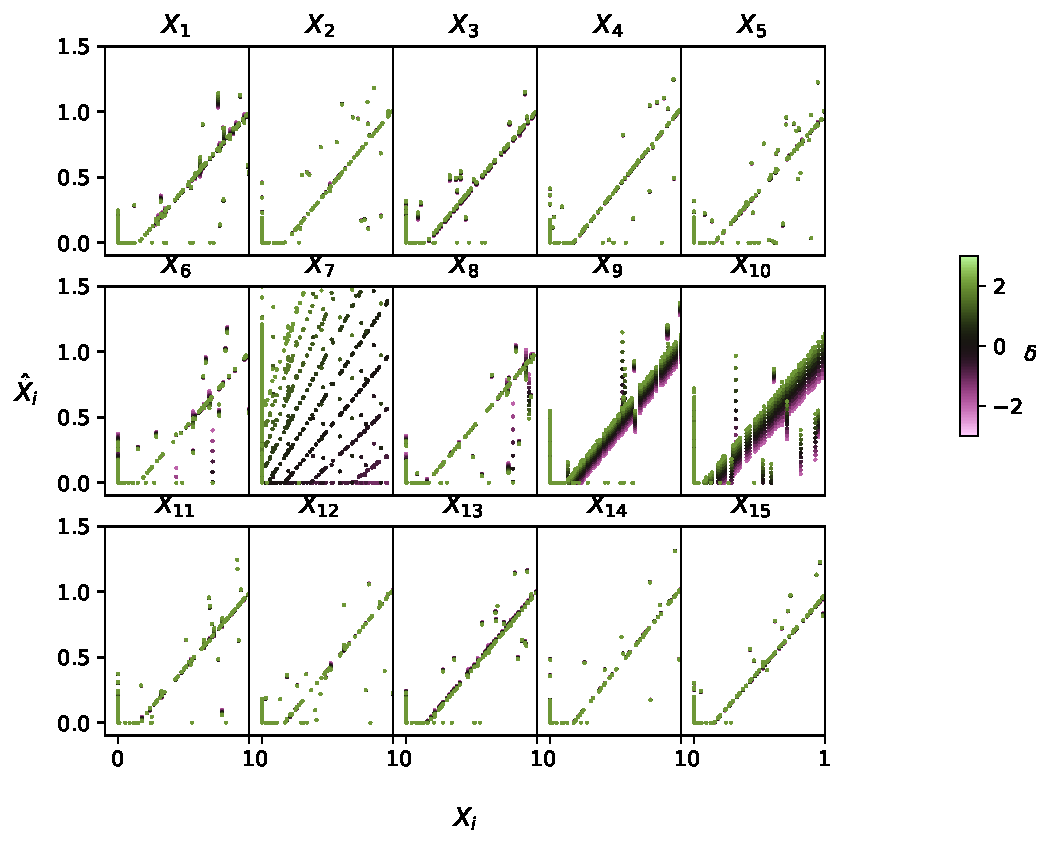
\includegraphics[width=\linewidth]{../figures/s4_tms_intervention_network4.pdf}
                \caption{Subnetwork 4}
            \end{subfigure} \\
            \hspace{\fill} % Spacer to align
            \begin{subfigure}{0.3\textwidth}
                \centering
                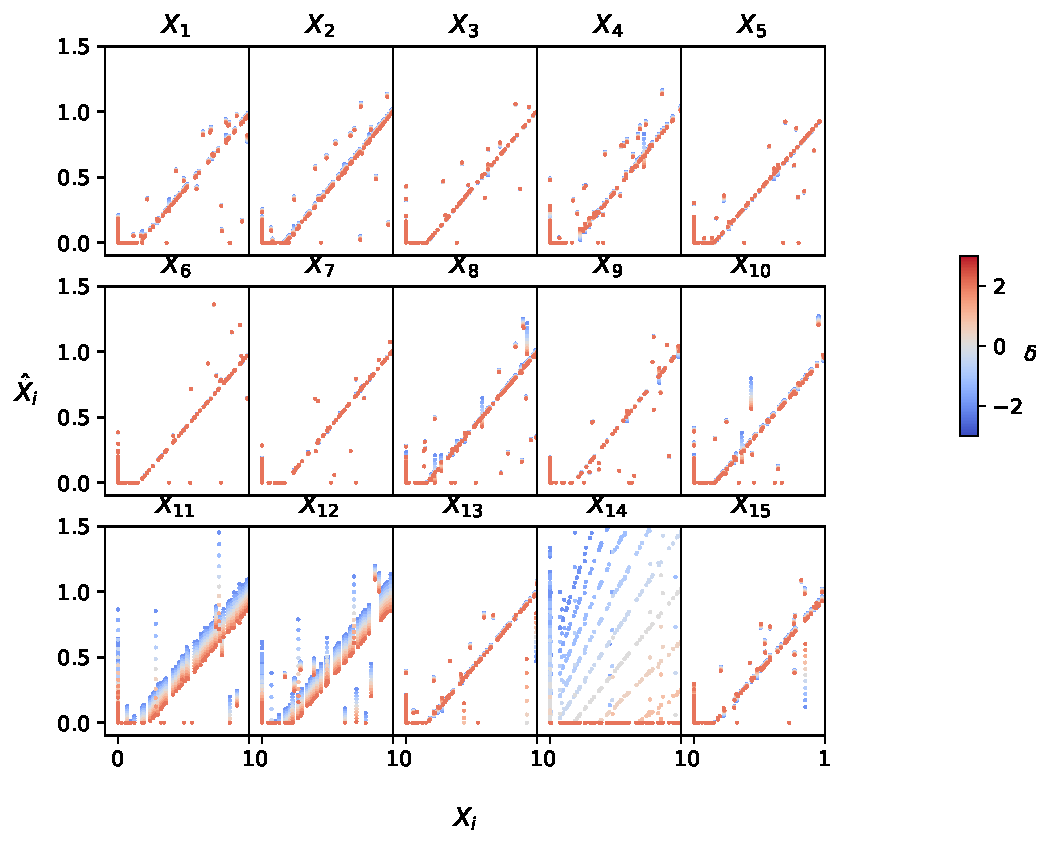
\includegraphics[width=\linewidth]{../figures/s4_tms_intervention_network5.pdf}
                \caption{Subnetwork 5}
            \end{subfigure} &
            \hspace{\fill} % Spacer to align
        \end{tabular}
    \end{minipage}

\end{figure}


%---------------- FIGURE S6: Higher Rank Circuit Superposition ----------------
\begin{figure}[ht]
    \centerline{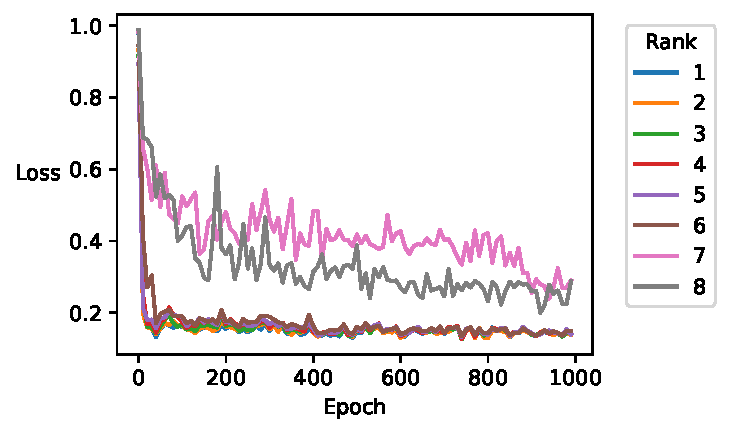
\includegraphics{../figures/s5_high_rank_circuits_loss_vs_rank.pdf}}
    \centering
    \caption{Loss vs Rank}\label{fig:s5_high_rank_circuits_loss_vs_rank}
\end{figure}

  
\begin{figure}[ht]
    \centering
    \caption{Decomposing the toy model of high rank circuits into different numbers of subnetworks}\label{fig:s6_high_rank_decompositions}
    \begin{minipage}{\textwidth} % Ensure figures align
        \centering
        \begin{tabular}{c}  % 3 columns
            \begin{subfigure}{0.3\textwidth}
                \centering
                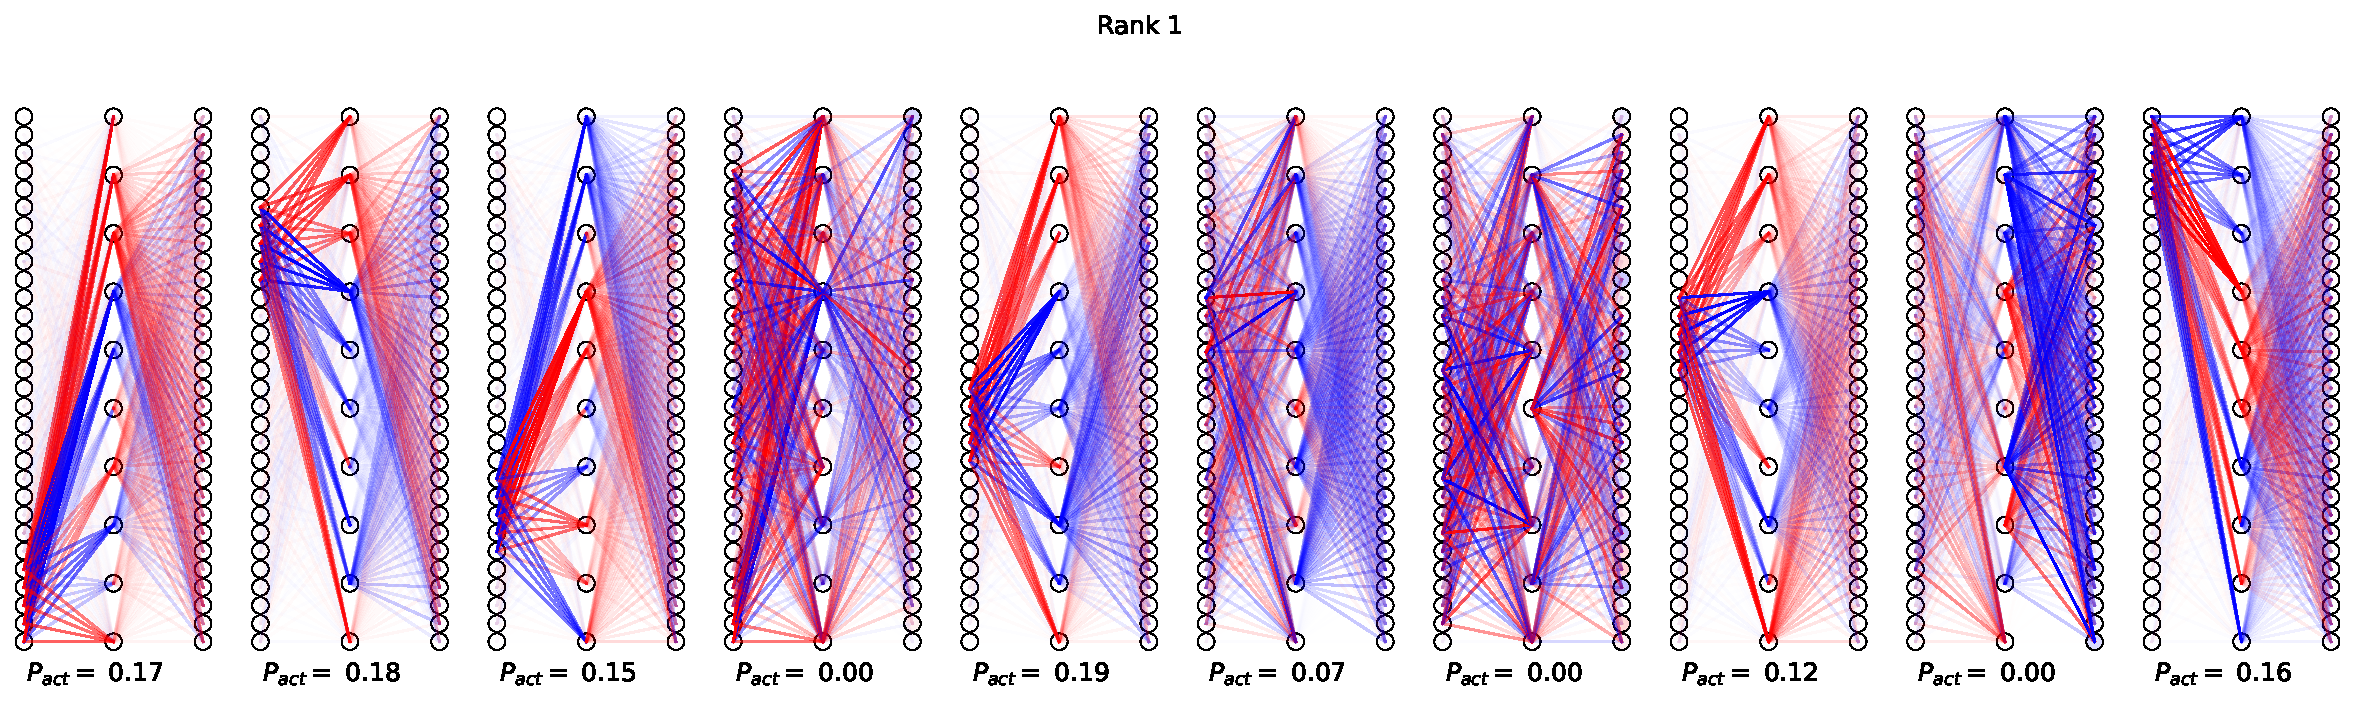
\includegraphics[width=\linewidth]{../figures/s6_high_rank_decompositions_rank1.pdf}
                \caption{Rank-1 Networks}
            \end{subfigure} \\
            \begin{subfigure}{0.3\textwidth}
                \centering
                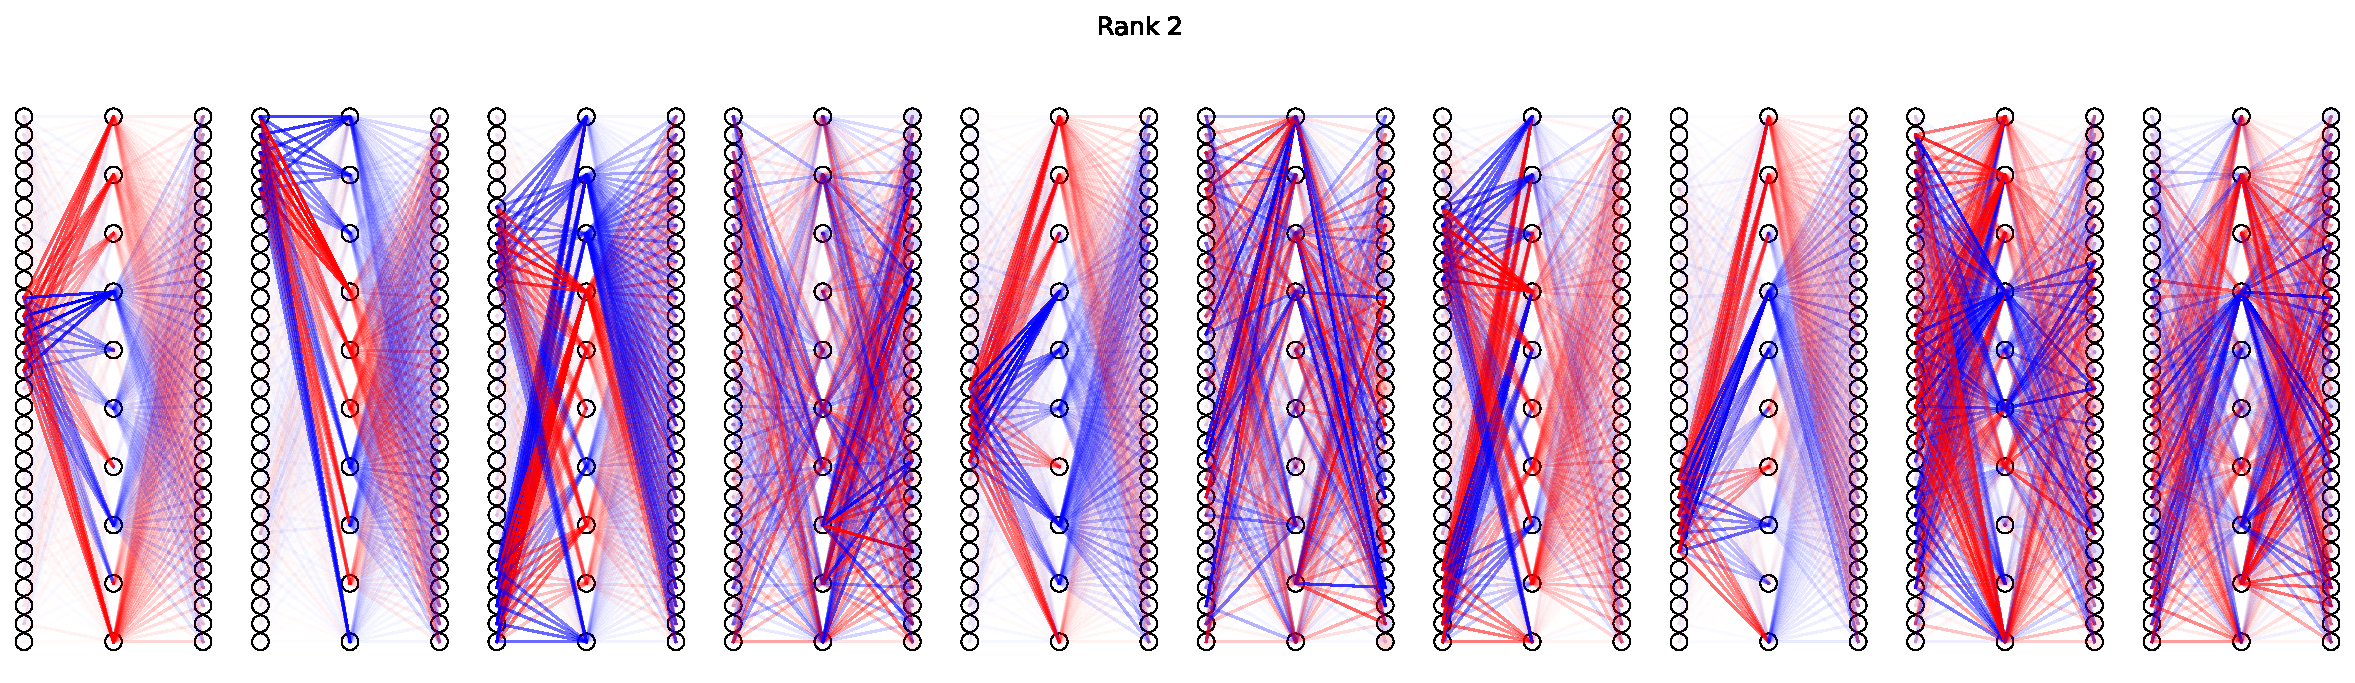
\includegraphics[width=\linewidth]{../figures/s6_high_rank_decompositions_rank2.pdf}
                \caption{Rank-2 Networks}
            \end{subfigure} \\
            \begin{subfigure}{0.3\textwidth}
                \centering
                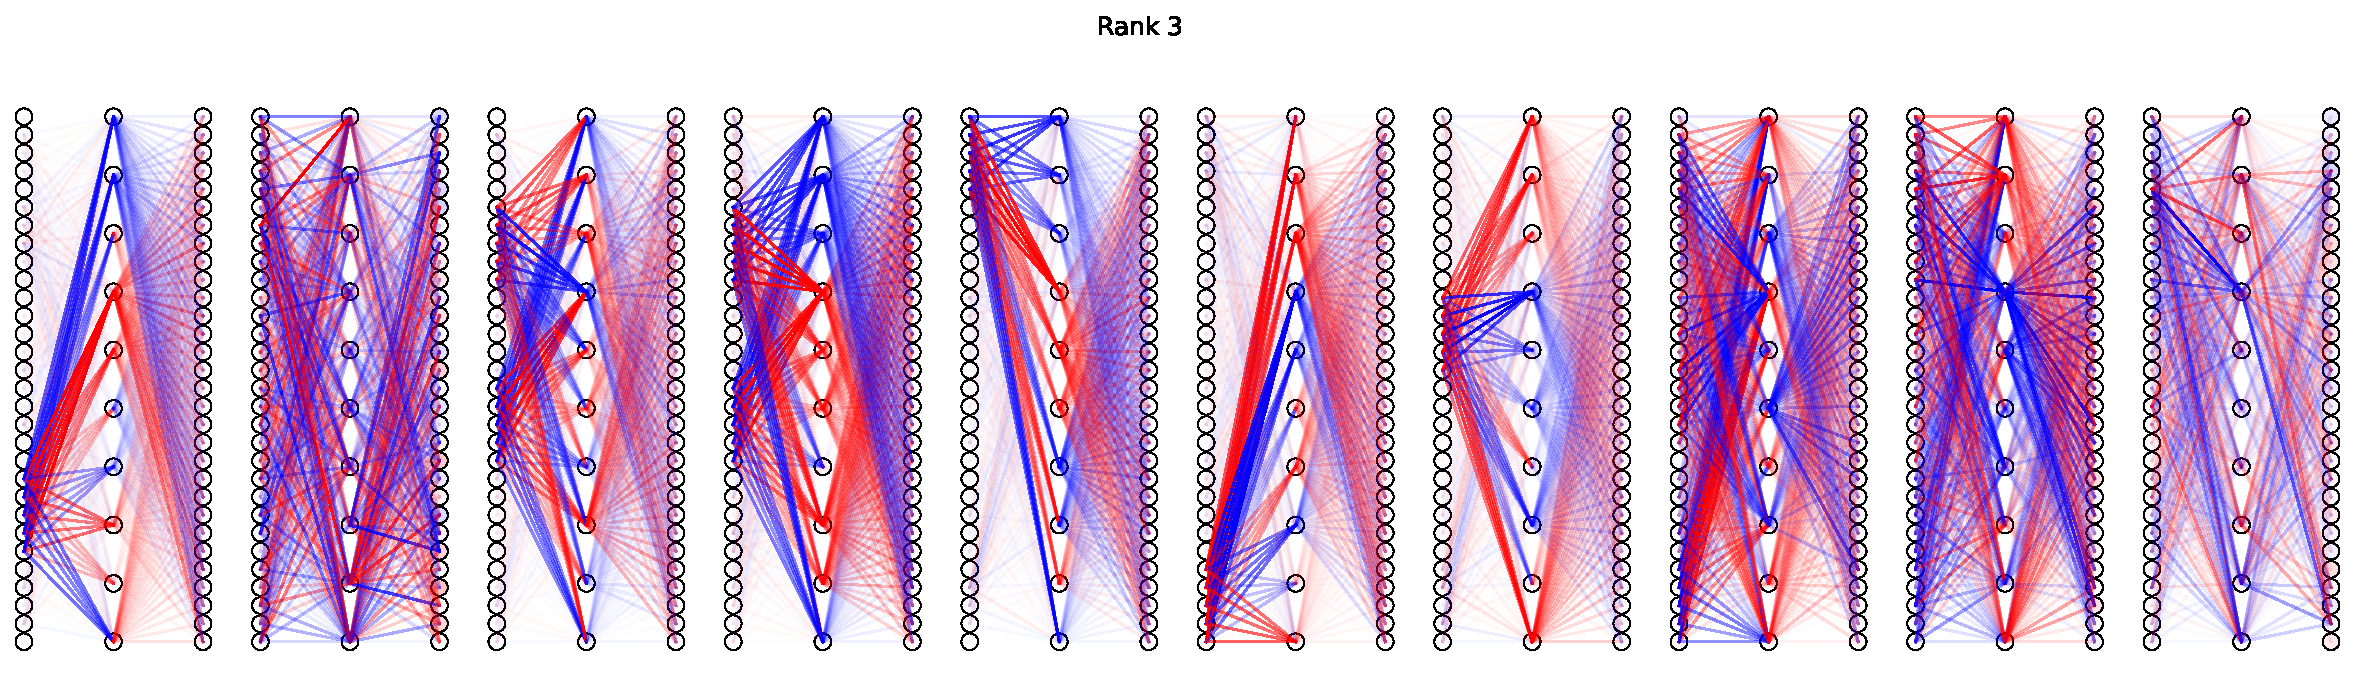
\includegraphics[width=\linewidth]{../figures/s6_high_rank_decompositions_rank3.pdf}
                \caption{Rank-3 Networks}
            \end{subfigure} \\
            \begin{subfigure}{0.3\textwidth}
                \centering
                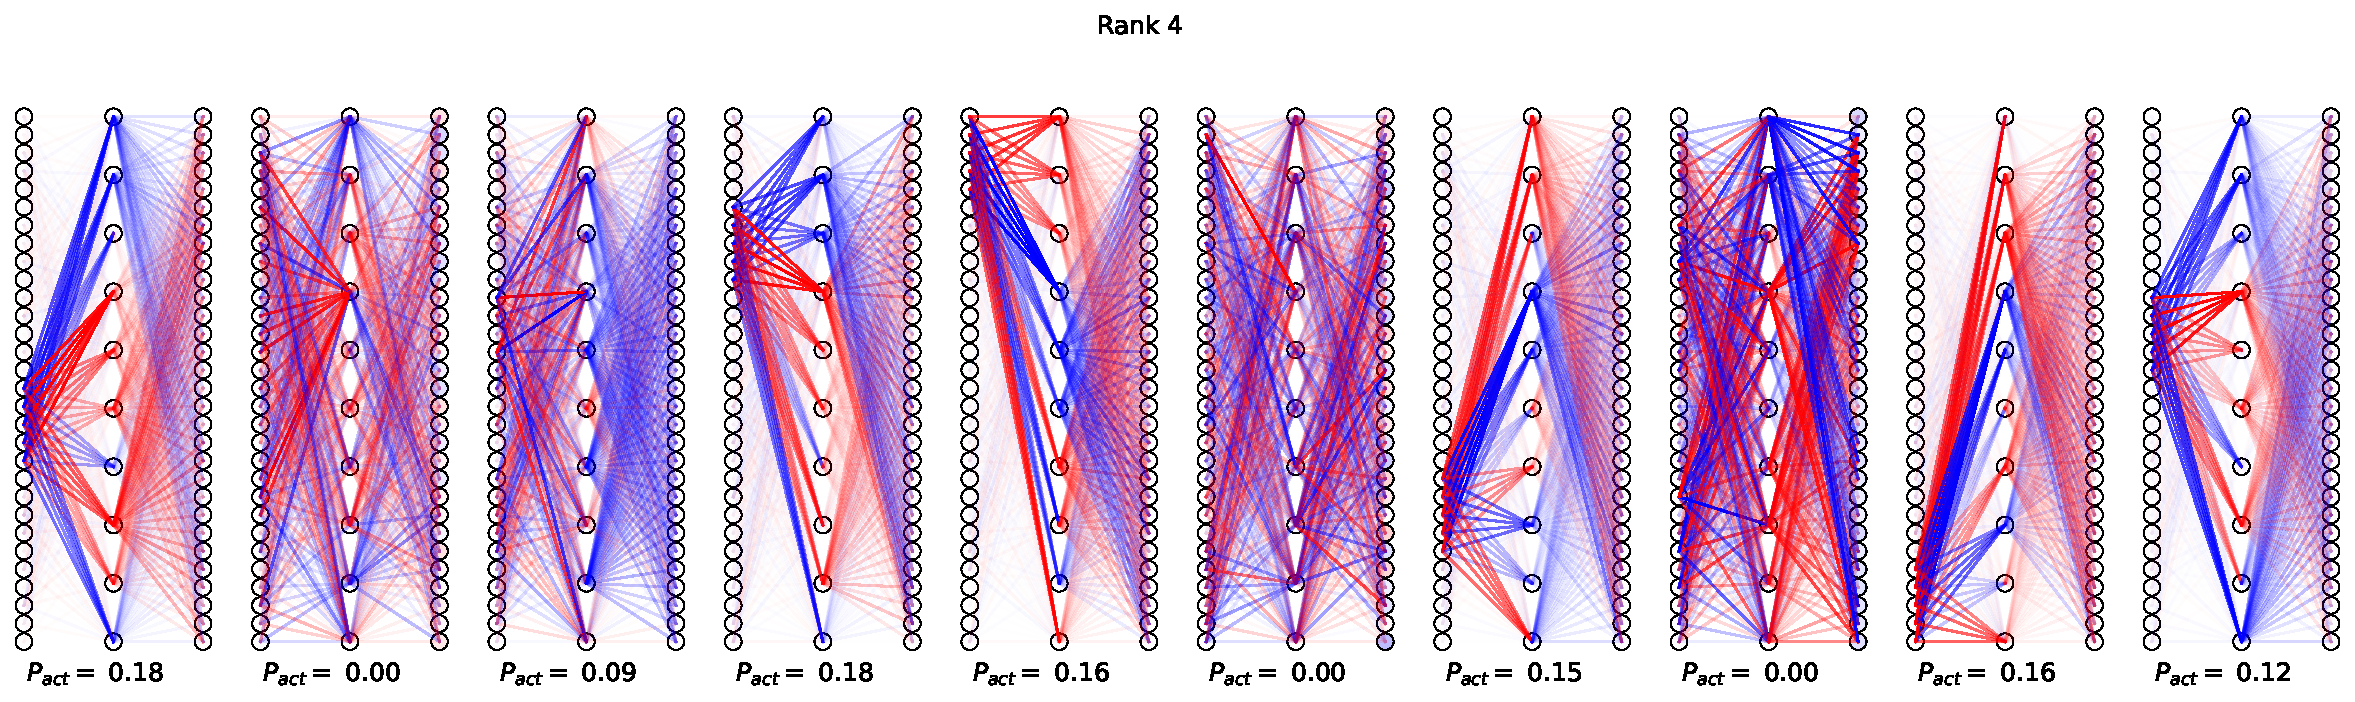
\includegraphics[width=\linewidth]{../figures/s6_high_rank_decompositions_rank4.pdf}
                \caption{Rank-4 Networks}
            \end{subfigure} \\
            \begin{subfigure}{0.3\textwidth}
                \centering
                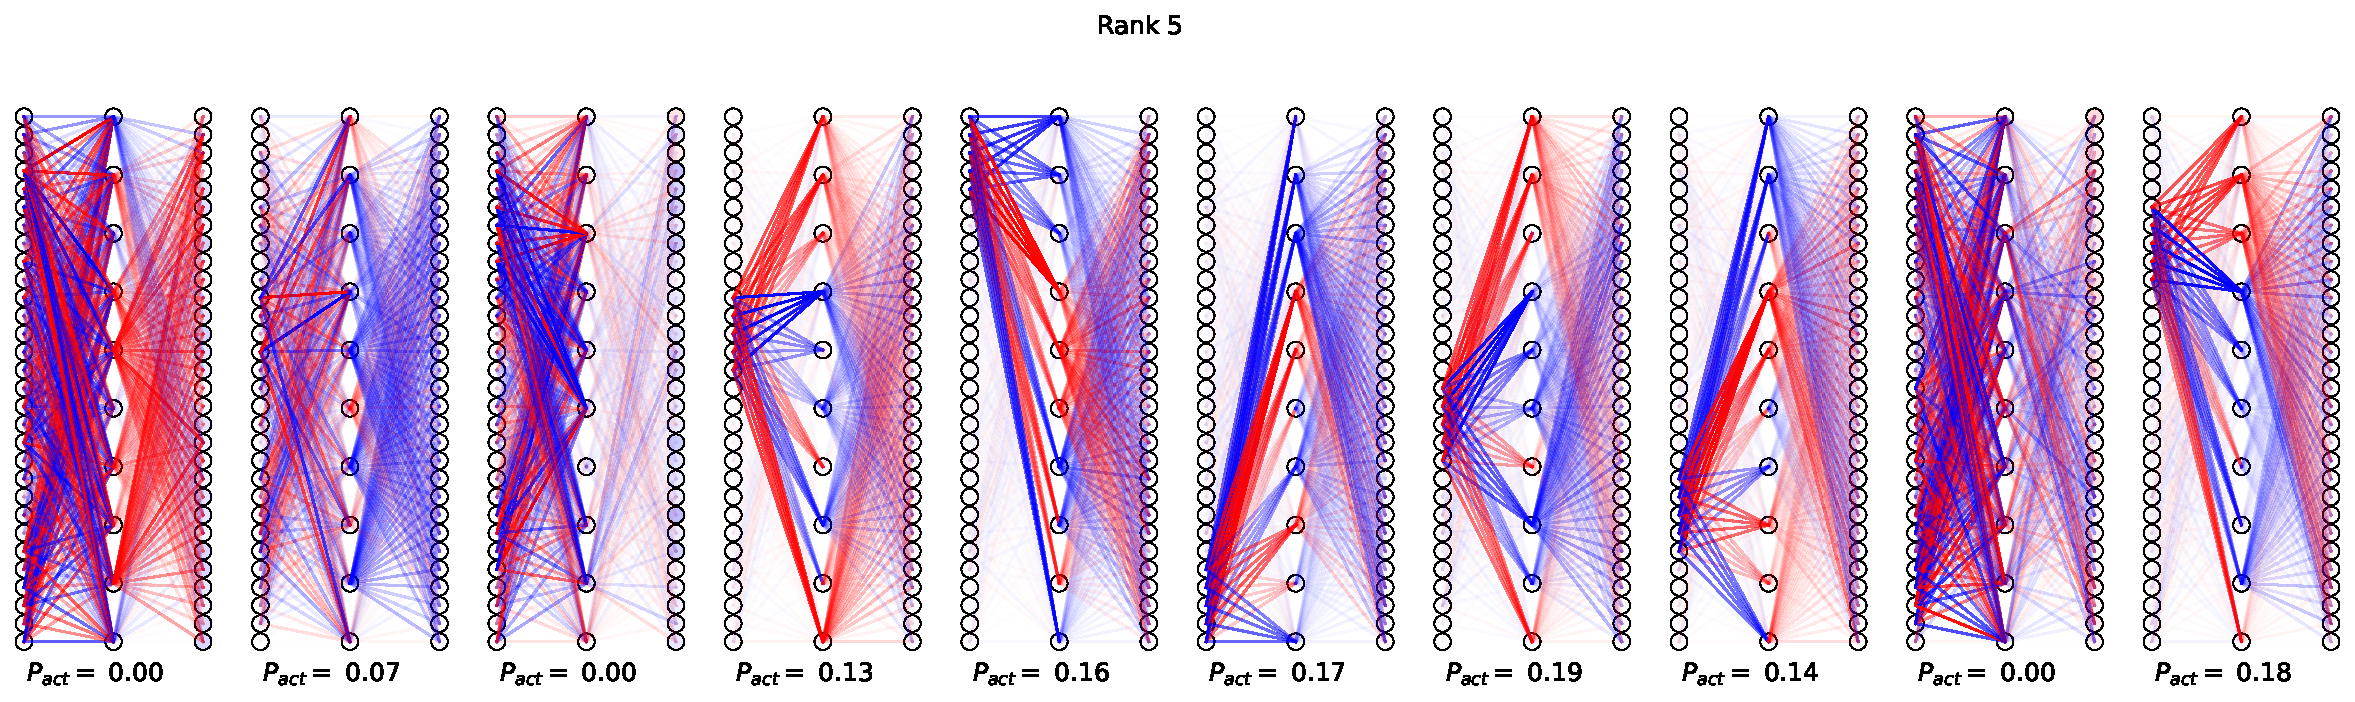
\includegraphics[width=\linewidth]{../figures/s6_high_rank_decompositions_rank5.pdf}
                \caption{Rank-5 Networks}
            \end{subfigure}  
        \end{tabular}
    \end{minipage}

\end{figure}

%--------------------- FIGURE S7: Squared Model More Deltas---------------------
\begin{figure}[ht]
    \centerline{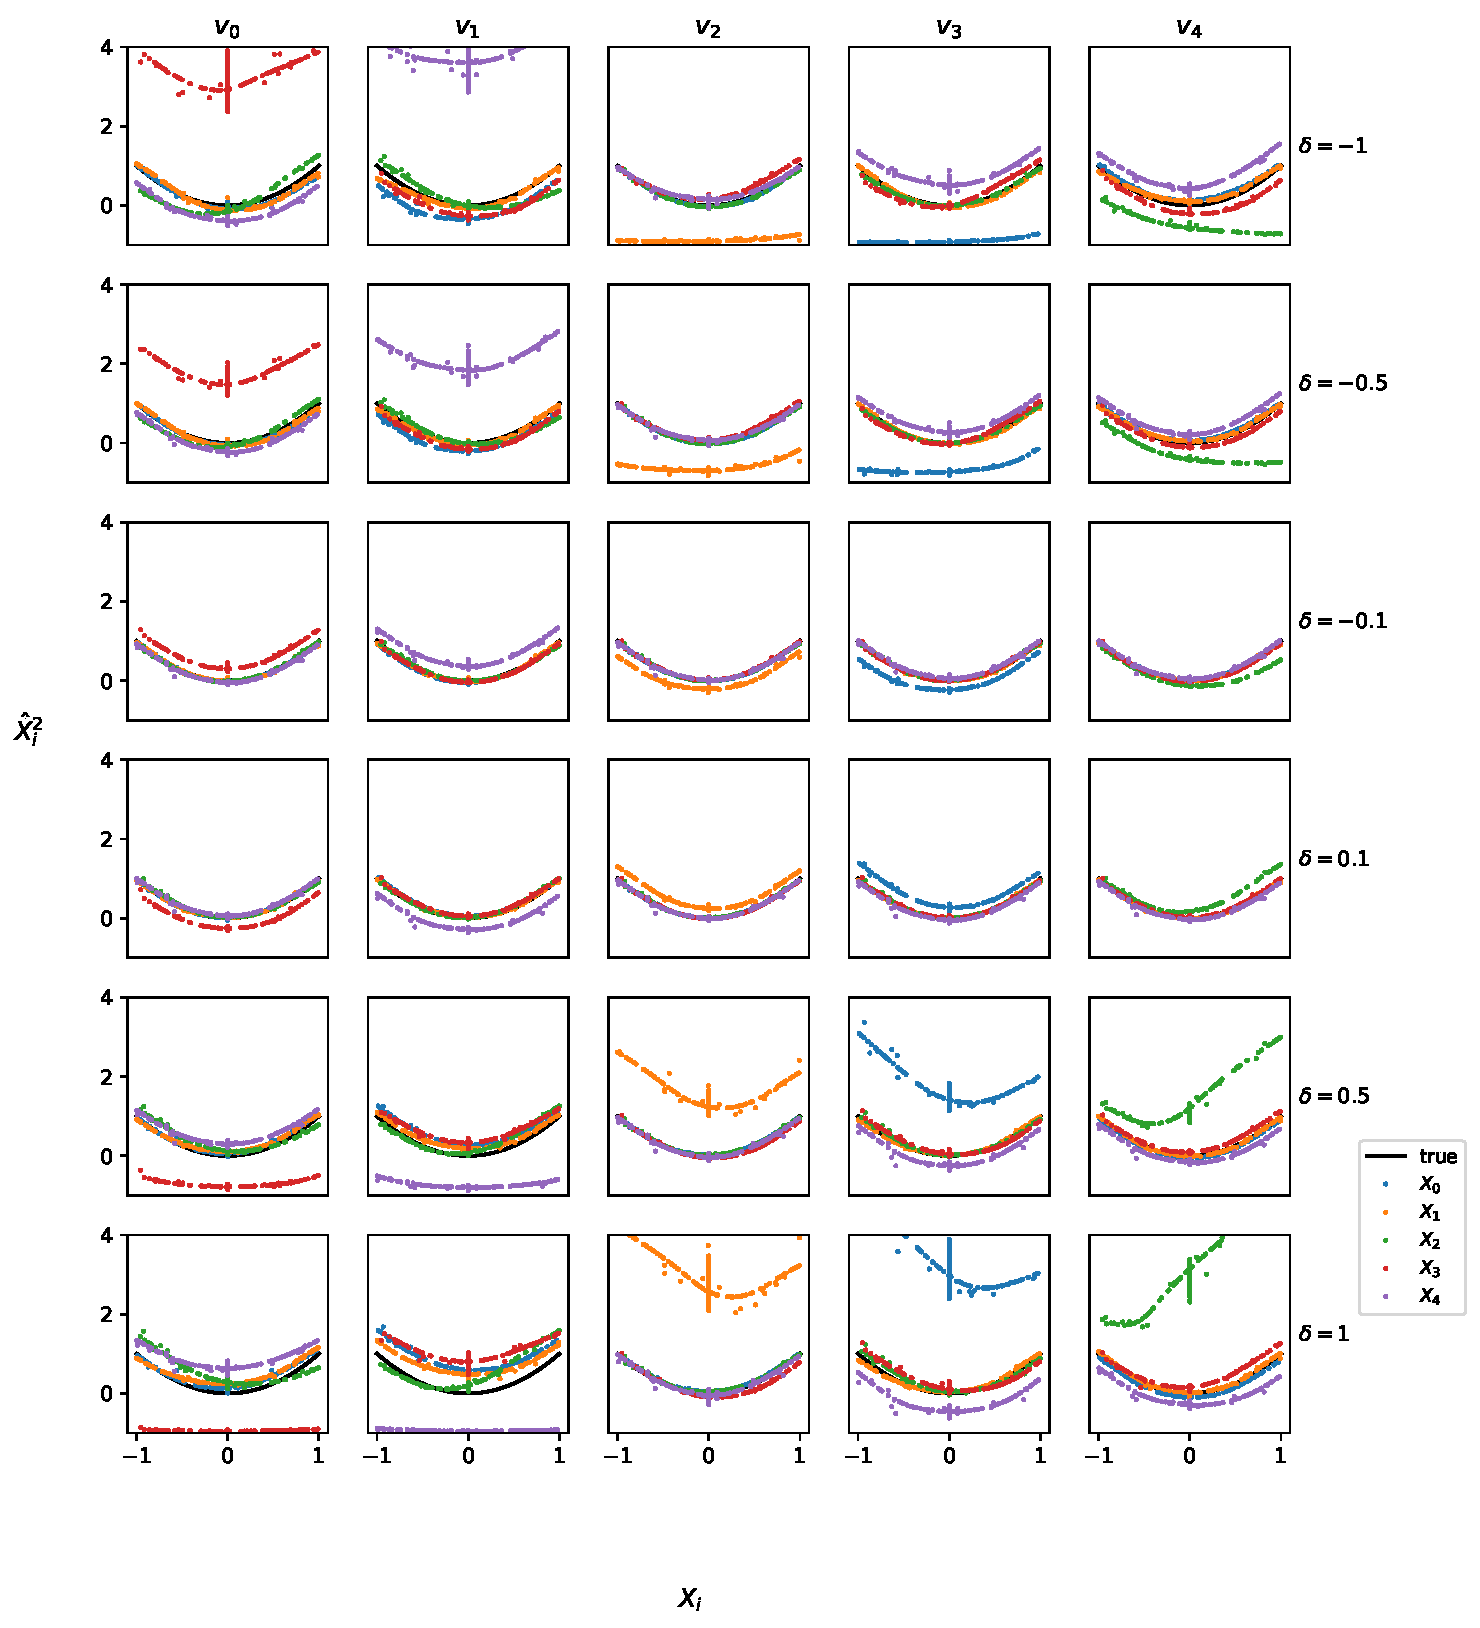
\includegraphics[width=\textwidth]{../figures/s7_squared_intervention_more_deltas.pdf}}
    \centering
    \caption{Effects of intervening on each of the subnetworks of the $X \mapsto X^2$ model.}\label{fig:s7_squared_intervention_more_deltas}
\end{figure}

%--------------------- FIGURE S8: Squared Model Middle Layer Intervention ---------------------
\begin{figure}[ht]
    \centerline{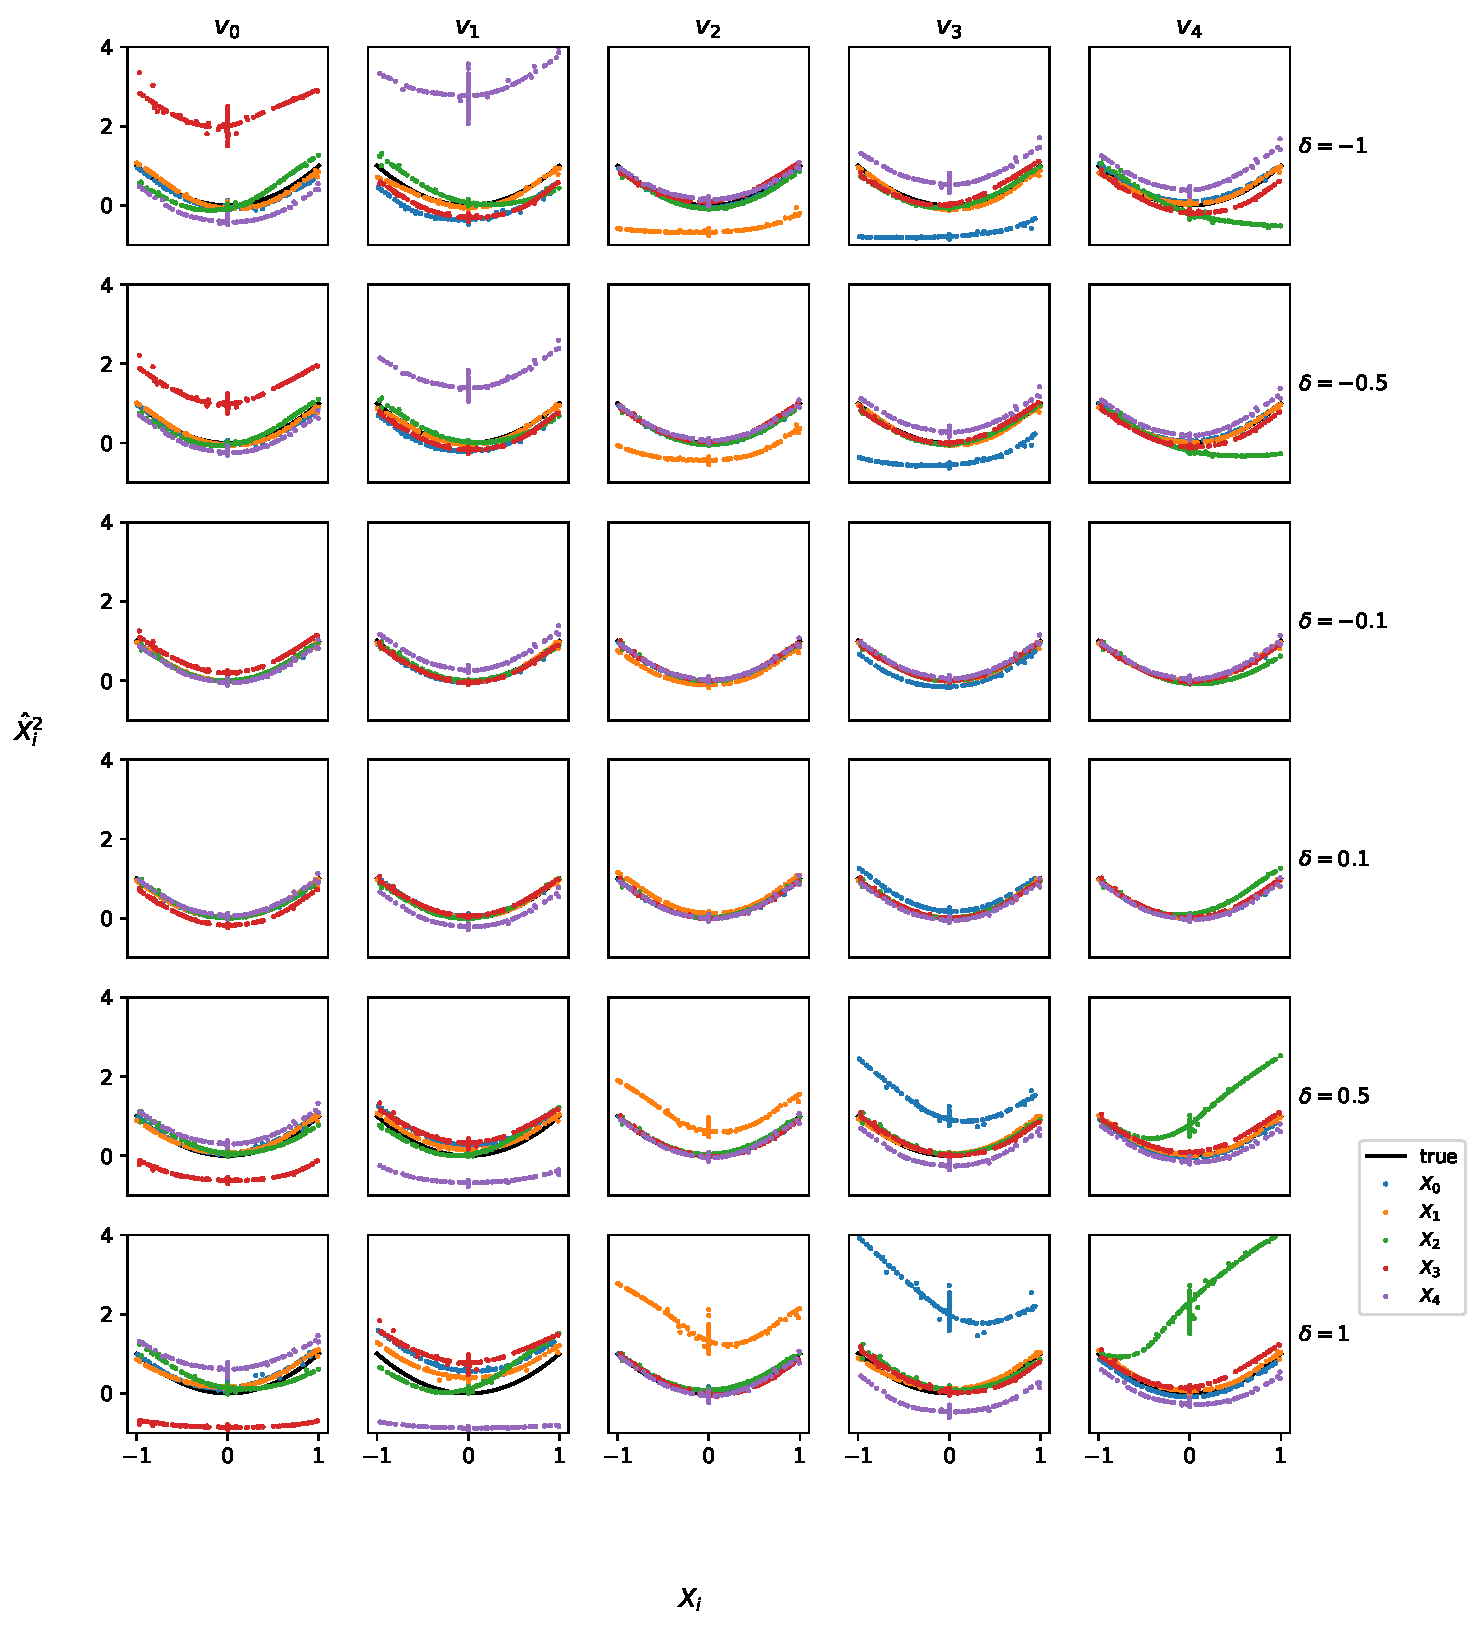
\includegraphics[width=\textwidth]{../figures/s8_squared_intervention_middle_weights.pdf}}
    \centering
    \caption{Effect of intervening using just the weights and biases of the middle hidden layers in the subnetworks of the $X \mapsto X^2$ model.}\label{fig:s8_squared_intervention_middle_weights}
\end{figure}


%--------------------- FIGURE S9: Squared Model Multi-Feature Intervention ---------------------
\begin{figure}[ht]
    \centerline{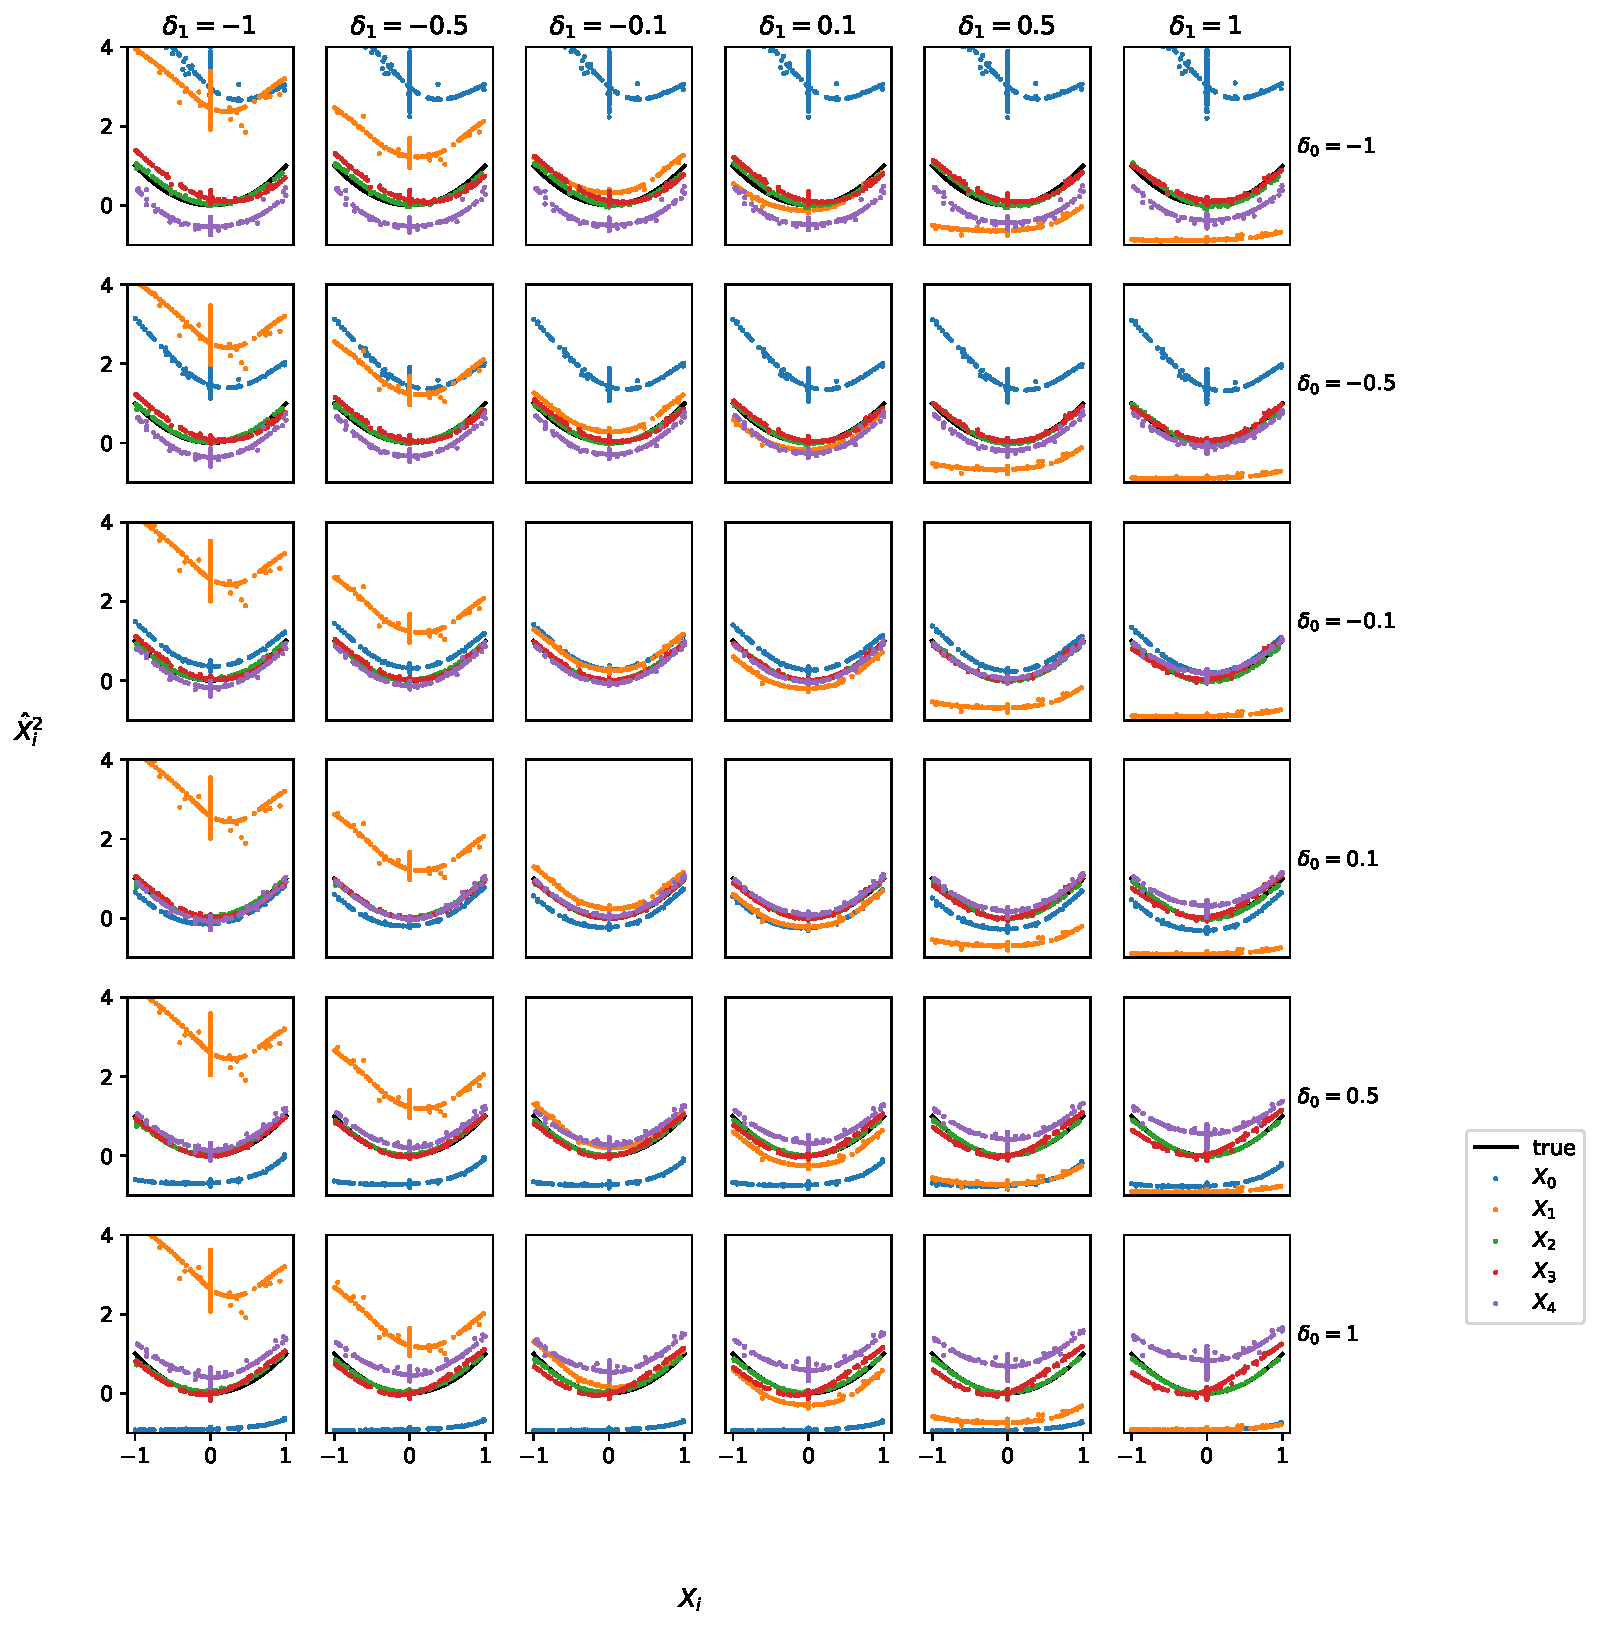
\includegraphics[width=\textwidth]{../figures/s9_squared_intervention_multi_features.pdf}}
    \centering
    \caption{Effects of intervening with multiple subnetworks ($v_0$ on the x-axis, $v_1$ on the y-axis) at once.}\label{fig:s9_squared_intervention_multi_features}
\end{figure}

%--------------------- FIGURE S10: Squared Model Decompositions ---------------------

% rootate this figure to landscape

\begin{figure}[ht]
    \centering
    \caption{Decomposing the $X \mapsto X^2$ model into different numbers of subnetworks}\label{fig:s10_squared_decompositions_features}
    \begin{minipage}{\textwidth} % Ensure figures align
        \centering
        \begin{tabular}{c}  % 3 columns
            \begin{subfigure}{0.3\textwidth}
                \centering
                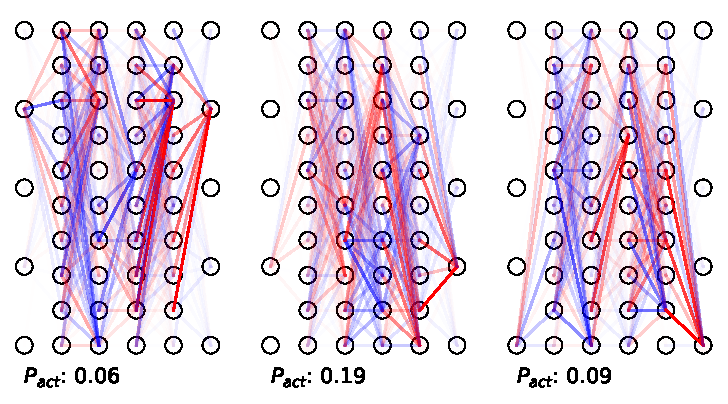
\includegraphics[width=\linewidth]{../figures/s10_squared_decompositions_feature3.pdf}
                \caption{3 rank-1 Networks}
            \end{subfigure} \\
            \begin{subfigure}{0.3\textwidth}
                \centering
                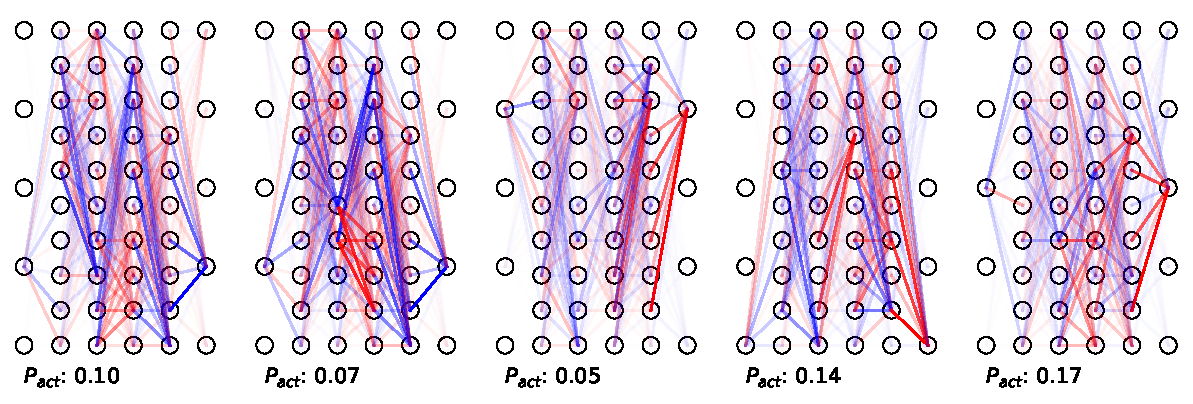
\includegraphics[width=\linewidth]{../figures/s10_squared_decompositions_feature5.pdf}
                \caption{5 rank-1 Networks}
            \end{subfigure} \\ % Move to the next row
            \begin{subfigure}{0.3\textwidth}
                \centering
                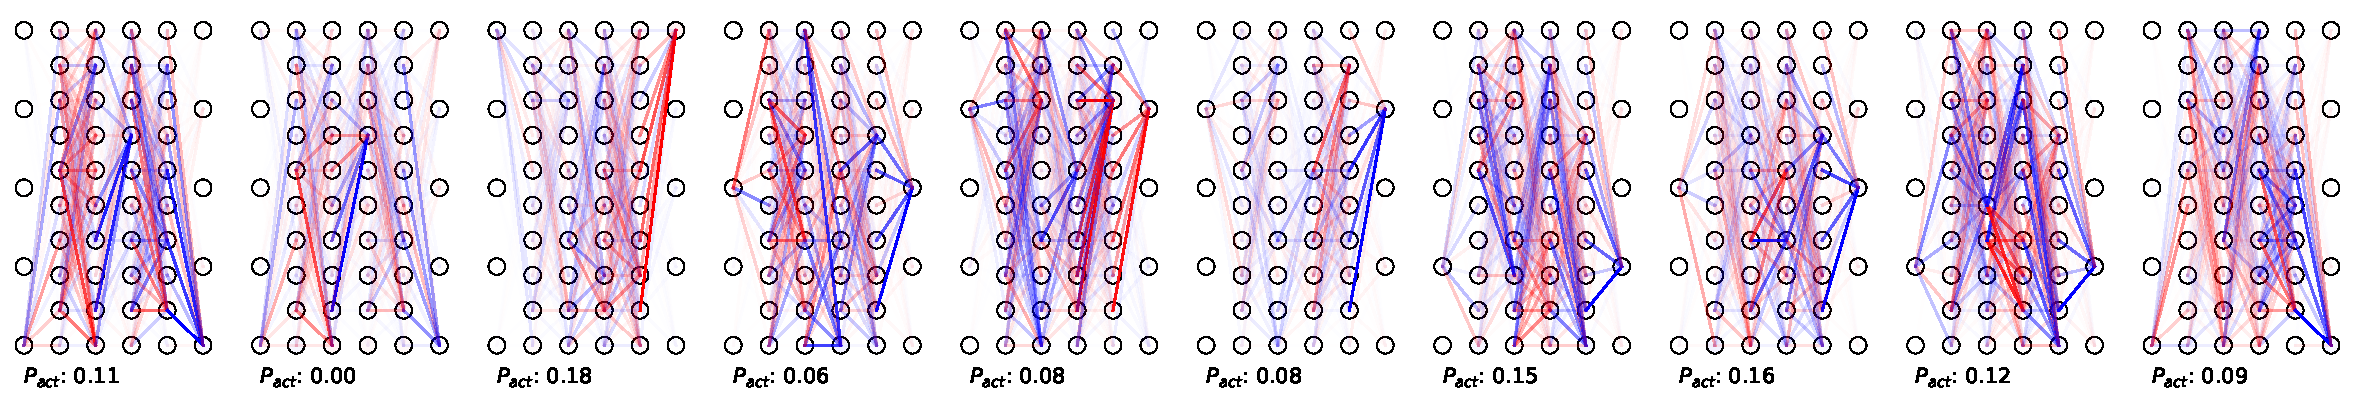
\includegraphics[width=\linewidth]{../figures/s10_squared_decompositions_feature10.pdf}
                \caption{10 rank-1 Networks}
            \end{subfigure} \\ % Move to the next row
            \begin{subfigure}{0.3\textwidth}
                \centering
                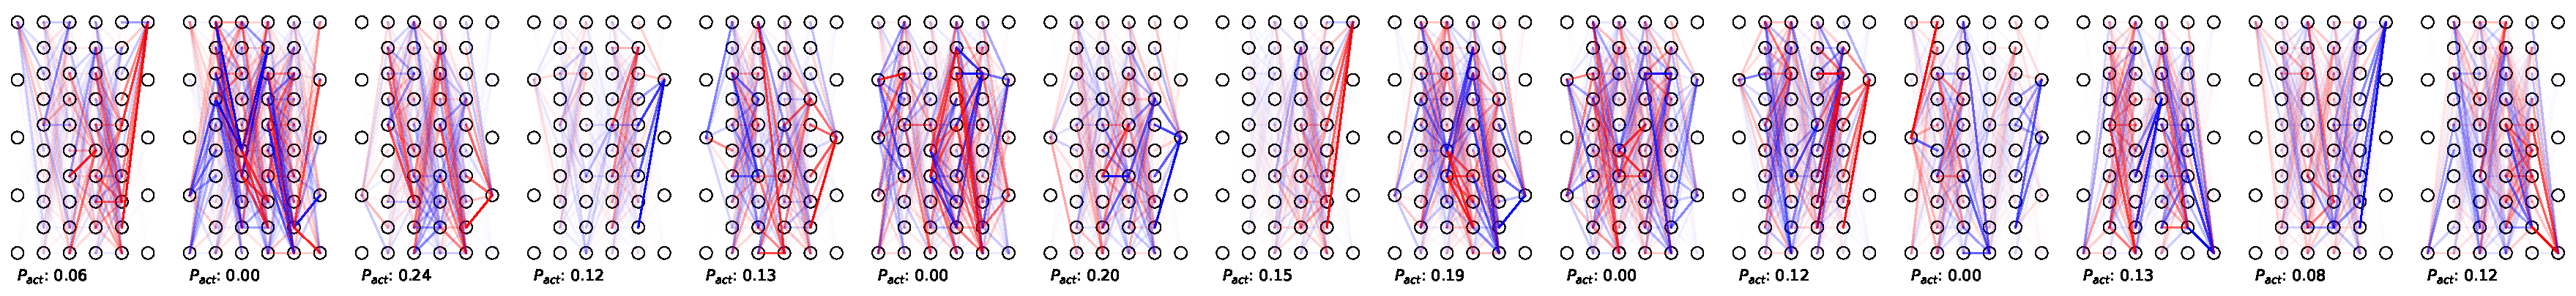
\includegraphics[width=\linewidth]{../figures/s10_squared_decompositions_feature15.pdf}
                \caption{15 rank-1 Networks}
            \end{subfigure} 
        \end{tabular}
    \end{minipage}

\end{figure}

%--------------------- FIGURE S11: Squared Model Loss Versus Rank ---------------------
\begin{figure}[ht]
    \centerline{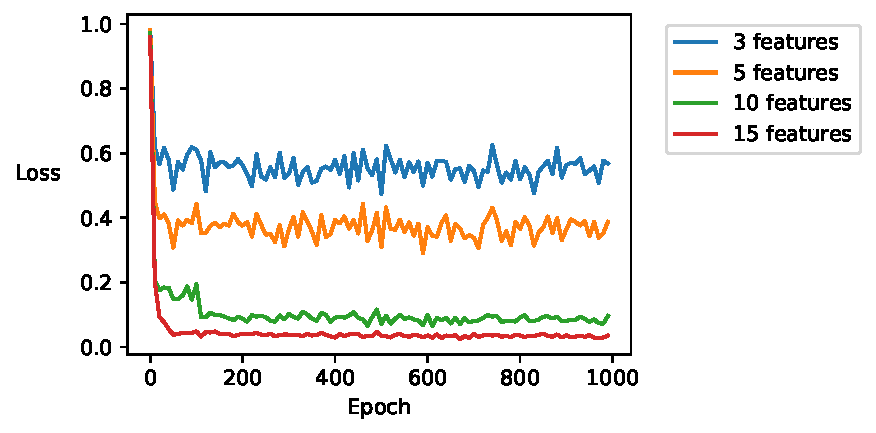
\includegraphics[width=\textwidth]{../figures/s11_squared_features_vs_loss.pdf}}
    \centering
    \caption{Training loss vs. number of subnetworks for the $X \mapsto X^2$ model}\label{fig:s11_squared_features_vs_loss}
\end{figure}

\end{document}